\chapter{Resultados}
\label{chap:res}

Como se indica en el secci\'on \ref{sec:genGrafFromImage}, la obtenci\'on de un grafo a partir de una imagen, es un proceso complejo. Las im\'agenes analizadas en este trabajo son aquellas en las que fue posible realizar el procedimiento de esqueletonizaci\'on, obteniendo un resultado que manten\'ia la topolog\'ia de la estructura original. Lo anterior no es un estado que pueda garantizarse para toda imagen. 


Los resultados que se presentan a continuaci\'on se separan entre tablas y figuras. Las tablas de resultados se encuentran dividas en 2 secciones dado el n\'umero de columnas. La primera secci\'on agrupa las m\'etricas y medidas indicadas en la secci\'on \ref{sec:metricasymedidas}. La segunda secci\'on muestra los porcentajes de cobertura y correctitud de los filamentos propuestos con respecto al {\it ground truth}.
Es necesario especificar que los porcentajes que se indican en la columna `` \% Cobertura de Aristas'' reflejan una condici\'on que no es una restricci\'on estricta del modelo o del algoritmo propuesto, a diferencia de DeFiNe, donde si se garantiza la cobertura de cada arista del grafo.


En cuanto a las figuras, el enfoque se dirige a presentar los resultados de DeFiNe y del algoritmo propuesto, con \'enfasis en los filamentos correctamente encontrados por uno de los algoritmos que el otro no haya podido individualizar. Cabe aclarar que el resultado gr\'afico al ejecutar DeFiNe realiza una rotaci\'on de 90\textdegree en sentido contrarreloj adem\'as de invertir el eje vertical. Ambas modificaciones han sido corregidas con el prop\'osito de comparar los resultados entre DeFiNe, el algoritmo propuesto y la individualizaci\'on de filamentos realizada por el experto.


En las mediciones del algoritmo propuesto, se muestra el promedio de las 5 iteraciones con diferentes semillas que se realizaron. El detalle de cada iteraci\'on, en conjunto con el c\'odigo y otros elementos necesarios para replicar estos resultados se encuentra en el \href{https://gitlab.com/LeoXDXp/graph-crawler}{repositorio github de esta tesis}. Parte de este detalle se incluye tambi\'en en el anexo \ref{chap:apendice}.
Las ejecuciones de DeFiNe y el algoritmo propuesto fueron realizadas en un computador con un procesador {\tt Intel i5-7200U} de 4 n\'ucleos, 8GB de RAM y un disco de estado s\'lido, bajo el sistema operativo {\tt Fedora 31}.

\section{Extracci\'o de un grafo desde una imagen}
\label{sec:graphImageExtraction}
La obtenci\'on de un grafo y la asociaci\'on de propiedades a sus nodos o aristas constituye el paso previo a la individualizaci\'on autom\'atica de filamentos. De acuerdo a lo descrito en la secci\'on \ref{subsec:infoLossSkel}, existen diversas formas para realizar este procedimiento. Para el caso de DeFiNe, sus autores indican que se preprocesa la imagen en escala de grises para resaltar las estructuras alargadas que debiesen ser filamentos, mediante un filtro de {\it veselness} y un umbral de mediana adaptativa. El paso siguiente consiste en realizar la esqueletonizaci\'on de la imagen, para luego construir un grafo en el que se asigna un peso a las aristas. 
Para obtener el peso de las aristas, se le aplica un filtro gaussiano a la imagen original en escala de grises, para luego promediar la intensidad a lo largo de cada arista.

% solo esta disponible el archivo GML para la imagen sintetica 1. No estan disponibles las imagenes base,

Una replica exacta de los pasos de aquel procedimiento no puede ser realizada, debido a que no se se\~nala el tama\~no del filtro gaussiano. Otro aspecto que dificulta una comparaci\'on directa es que DeFiNe no considera la curvatura de las aristas, sino que solo las representa como lineas rectas mediante la conexión punto a punto entre los nodos. Adicionalmente, no se encontraron las im\'agenes originales utilizadas en aqueela investigaci\'on. Lo anterior implica que la solo se pudo realizar una comparaci\'on entre DeFiNe y el algoritmo propuesto, utilizando el \'unico ejemplo que trae DeFiNe, que corresponde al grafo ponderado con el que se realiza la individualizaci\'on de filamentos de la Figura 1b de aquella investigaci\'on, a partir de la cual se extrae una secci\'on, representada en la Figura \ref{fig:synth-Define-1b}.


En los otros casos donde se utiliza DeFiNe para obtener una individualizaci\'on de filamentos, se extrae el grafo necesario utilizando la herramienta {\it sknw}, la que pondera cada arista con su respectivo largo, el cual s\'i considera la curvatura. Este enfoque es compatible con lo que se presenta en \cite{breuer2015define}, ya que se indica que el m\'etodo utilizado por DeFiNe sirve para cualquier red ponderada extra\'ida a partir de una imagen.


\section{Im\'agenes Sint\'eticas}

%Resultados Synth QFS
Los resultados de la individualizaci\'on automatizada de filamentos sint\'eticos en la Figura \ref{fig:synth-QFS-7} se indican en la Tabla \ref{tab:synth-QFS-7-Results}. DeFiNe logra 4 de 6 individualizaciones al utilizar 30\textdegree, mientras que con 60\textdegree obtiene 3 de 6. Este \'ultimo resultado es el mismo que se obtiene en todas las iteraciones del algoritmo propuesto. La comparaci\'on entre los filamentos propuestos por cada m\'etodo y los correctamente identificados se observa en la Figura \ref{fig:Synth-QIFS-Result}.


En este caso de filamentos sint\'eticos, el filamento azul observable en la Figura \ref{fig:synth-QFS-7-gt}, corresponde a una sola arista del grafo (Figura \ref{fig:synth-QFS-7-graph}), por lo que tambi\'en en todas las pruebas con DeFiNe y con el algoritmo propuesto se obtiene para ese filamento un calce no exacto. Este calce no exacto no se considera una respuesta correcta, pero representa una situaci\'on que puede suceder en im\'agenes reales. En particular, se sobre-representa el filamento al agregar una arista del filamento vecino, de color celeste.


Ambas ejecuciones de DeFiNe, as\'i como todas las ejecuciones del algoritmo propuesto logran asignar cada arista a al menos un camino que representa un filamento. Este comportamiento es obligatorio para el m\'etodo de DeFiNe pero no para el algoritmo propuesto.


%%%% Como explicar VI, Rand y Jaccard, y los otros numeros
....

\begin{table}[t]
    \centering
    \begin{tabular}{|c|c|c|c|c|c|c|c|c|c|c|}
    \hline
        Algoritmo & VI & TP & FP &TN &FN & Rand	& Jaccard &	Precision &	Recall &	F1 \\ \hline
        DeFiNe 30\textdegree & 0.7958 & 8 & 3 & 58 & 9 & 0.8461 & 0.4    & 0.7272 & 0.4705 & 0.5714 \\
        DeFiNe 60\textdegree & 0.9777 & 7 & 4 & 50 & 5 & 0.8636 & 0.4375 & 0.6363 & 0.5833 & 0.6086  \\
        Propuesta & 1.6360 & 10.8 & 10.4 & 104.8 & 28 & 0.7646 & 0.2484 & 0.5142 & 0.3289 & 0.3919 \\
        \hline
    \end{tabular}
    \caption{M\'etricas y medidas en la individualizaci\'on de filamentos de la figura \ref{fig:synth-QFS-7}. .....El valor m\'aximo de VI en este caso es de 2.397895, con un {\it data set} de 11 aristas. El n\'umero de filamentos en el {\it ground truth} es 6.}
    \label{tab:synth-QFS-7-Results}
\end{table}
\addtocounter{table}{-1}
\begin{table}[h]
    \centering
    \begin{tabular}{|c|c|c|c|c|c|c|}
    \hline
         & \multirow{4}{2cm}{\centering \% Cobertura de Aristas} & \multirow{4}{2cm}{Filamentos Propuestos} & \multirow{4}{2cm}{Filamentos Correctos} & \multirow{4}{2.5cm}{\% Correctos vs Propuestos} & \multirow{4}{2.5cm}{\centering \% Correctos vs {\it Ground Truth}} & \multirow{4}{1.2cm}{\centering Tiempo [seg]} \\
         &  &  &  & & &  \\
        Algoritmo &  &  &  & & &  \\
        &  &  &  & & &  \\ \hline
        Define 30° & 100 & 6  & 4 & 66.6667 & 66.6667 & 2.3128 \\
        Define 60° & 100 & 5  & 3 & 60 & 50 & 2.338012\\ 
        Propuesta & 100 & 6.2 & 3 & 49.1428 & 50 & 0.3569\\
        \hline
    \end{tabular}
    \caption{Resultados del n\'umero de filamentos individualizados en la figura \ref{fig:synth-QFS-7}. ...El n\'umero de filamentos en el {\it ground truth} es 6.}
    %\label{tab:synth-QFS-7-Results2}
\end{table}


\begin{figure*}[h!]
    \centering
    \begin{subfigure}[t]{0.49\textwidth}
        \centering
        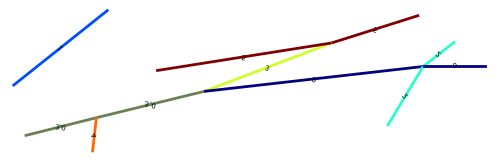
\includegraphics[scale=0.6]{resultImages/Synth-QFS-Fig7-Define30.png}
        \caption{Individualizaci\'on de filamenots de DeFiNe con 30\textdegree .}
        \label{fig:}
    \end{subfigure}%
    ~ 
    \begin{subfigure}[t]{0.49\textwidth}
        \centering
        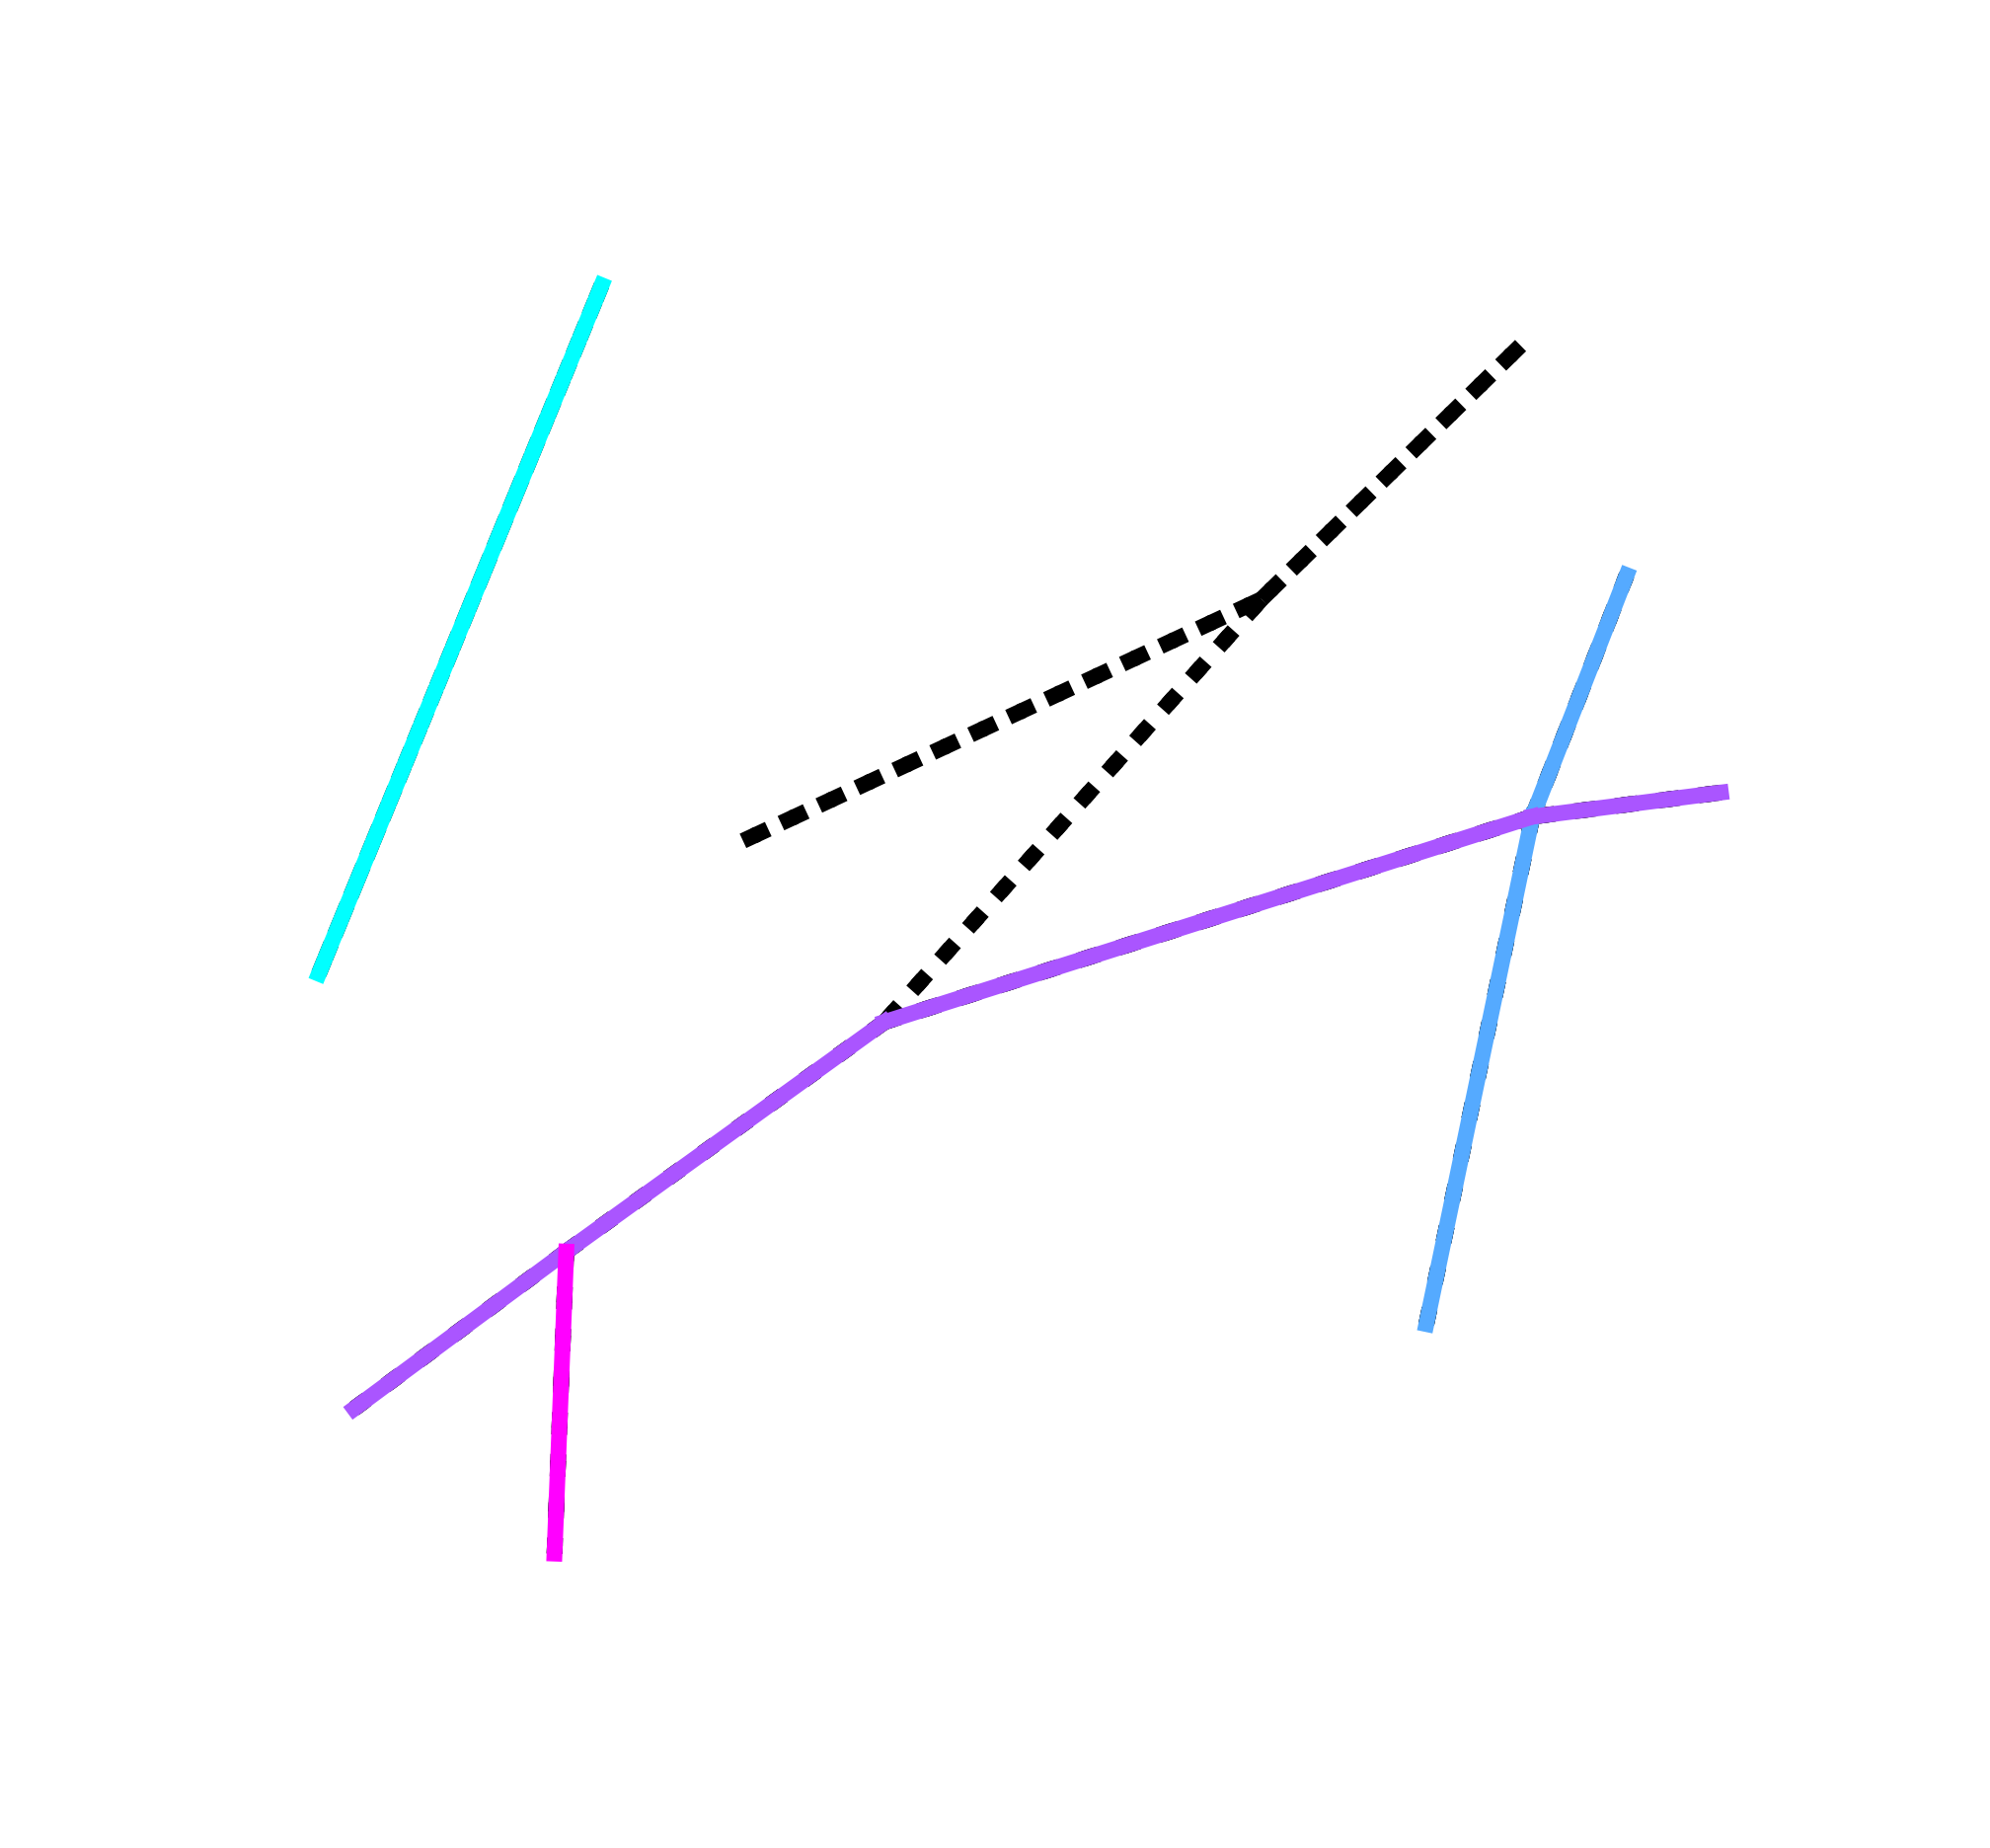
\includegraphics[height=1.5in]{resultImages/QFS7-DeFiNeExactMatch-30.png}
        \caption{4 filamentos correctamente individualizados por DeFiNe con 30\textdegree .}
        \label{fig:SpinningMarchantiaResults-define30Exact}
    \end{subfigure}
    \vskip\baselineskip
    
    \begin{subfigure}[t]{0.49\textwidth}
        \centering
        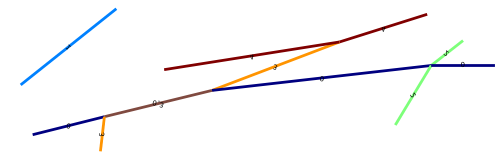
\includegraphics[scale=0.6]{resultImages/Synth-QFS-Fig7-Define60.png}
        \caption{Individualizaci\'on de filamenots mediante DeFiNe con 60\textdegree .}
        \label{fig:SpinningMarchantiaResults-define60}
    \end{subfigure}
    ~ 
    \begin{subfigure}[t]{0.49\textwidth}
        \centering
        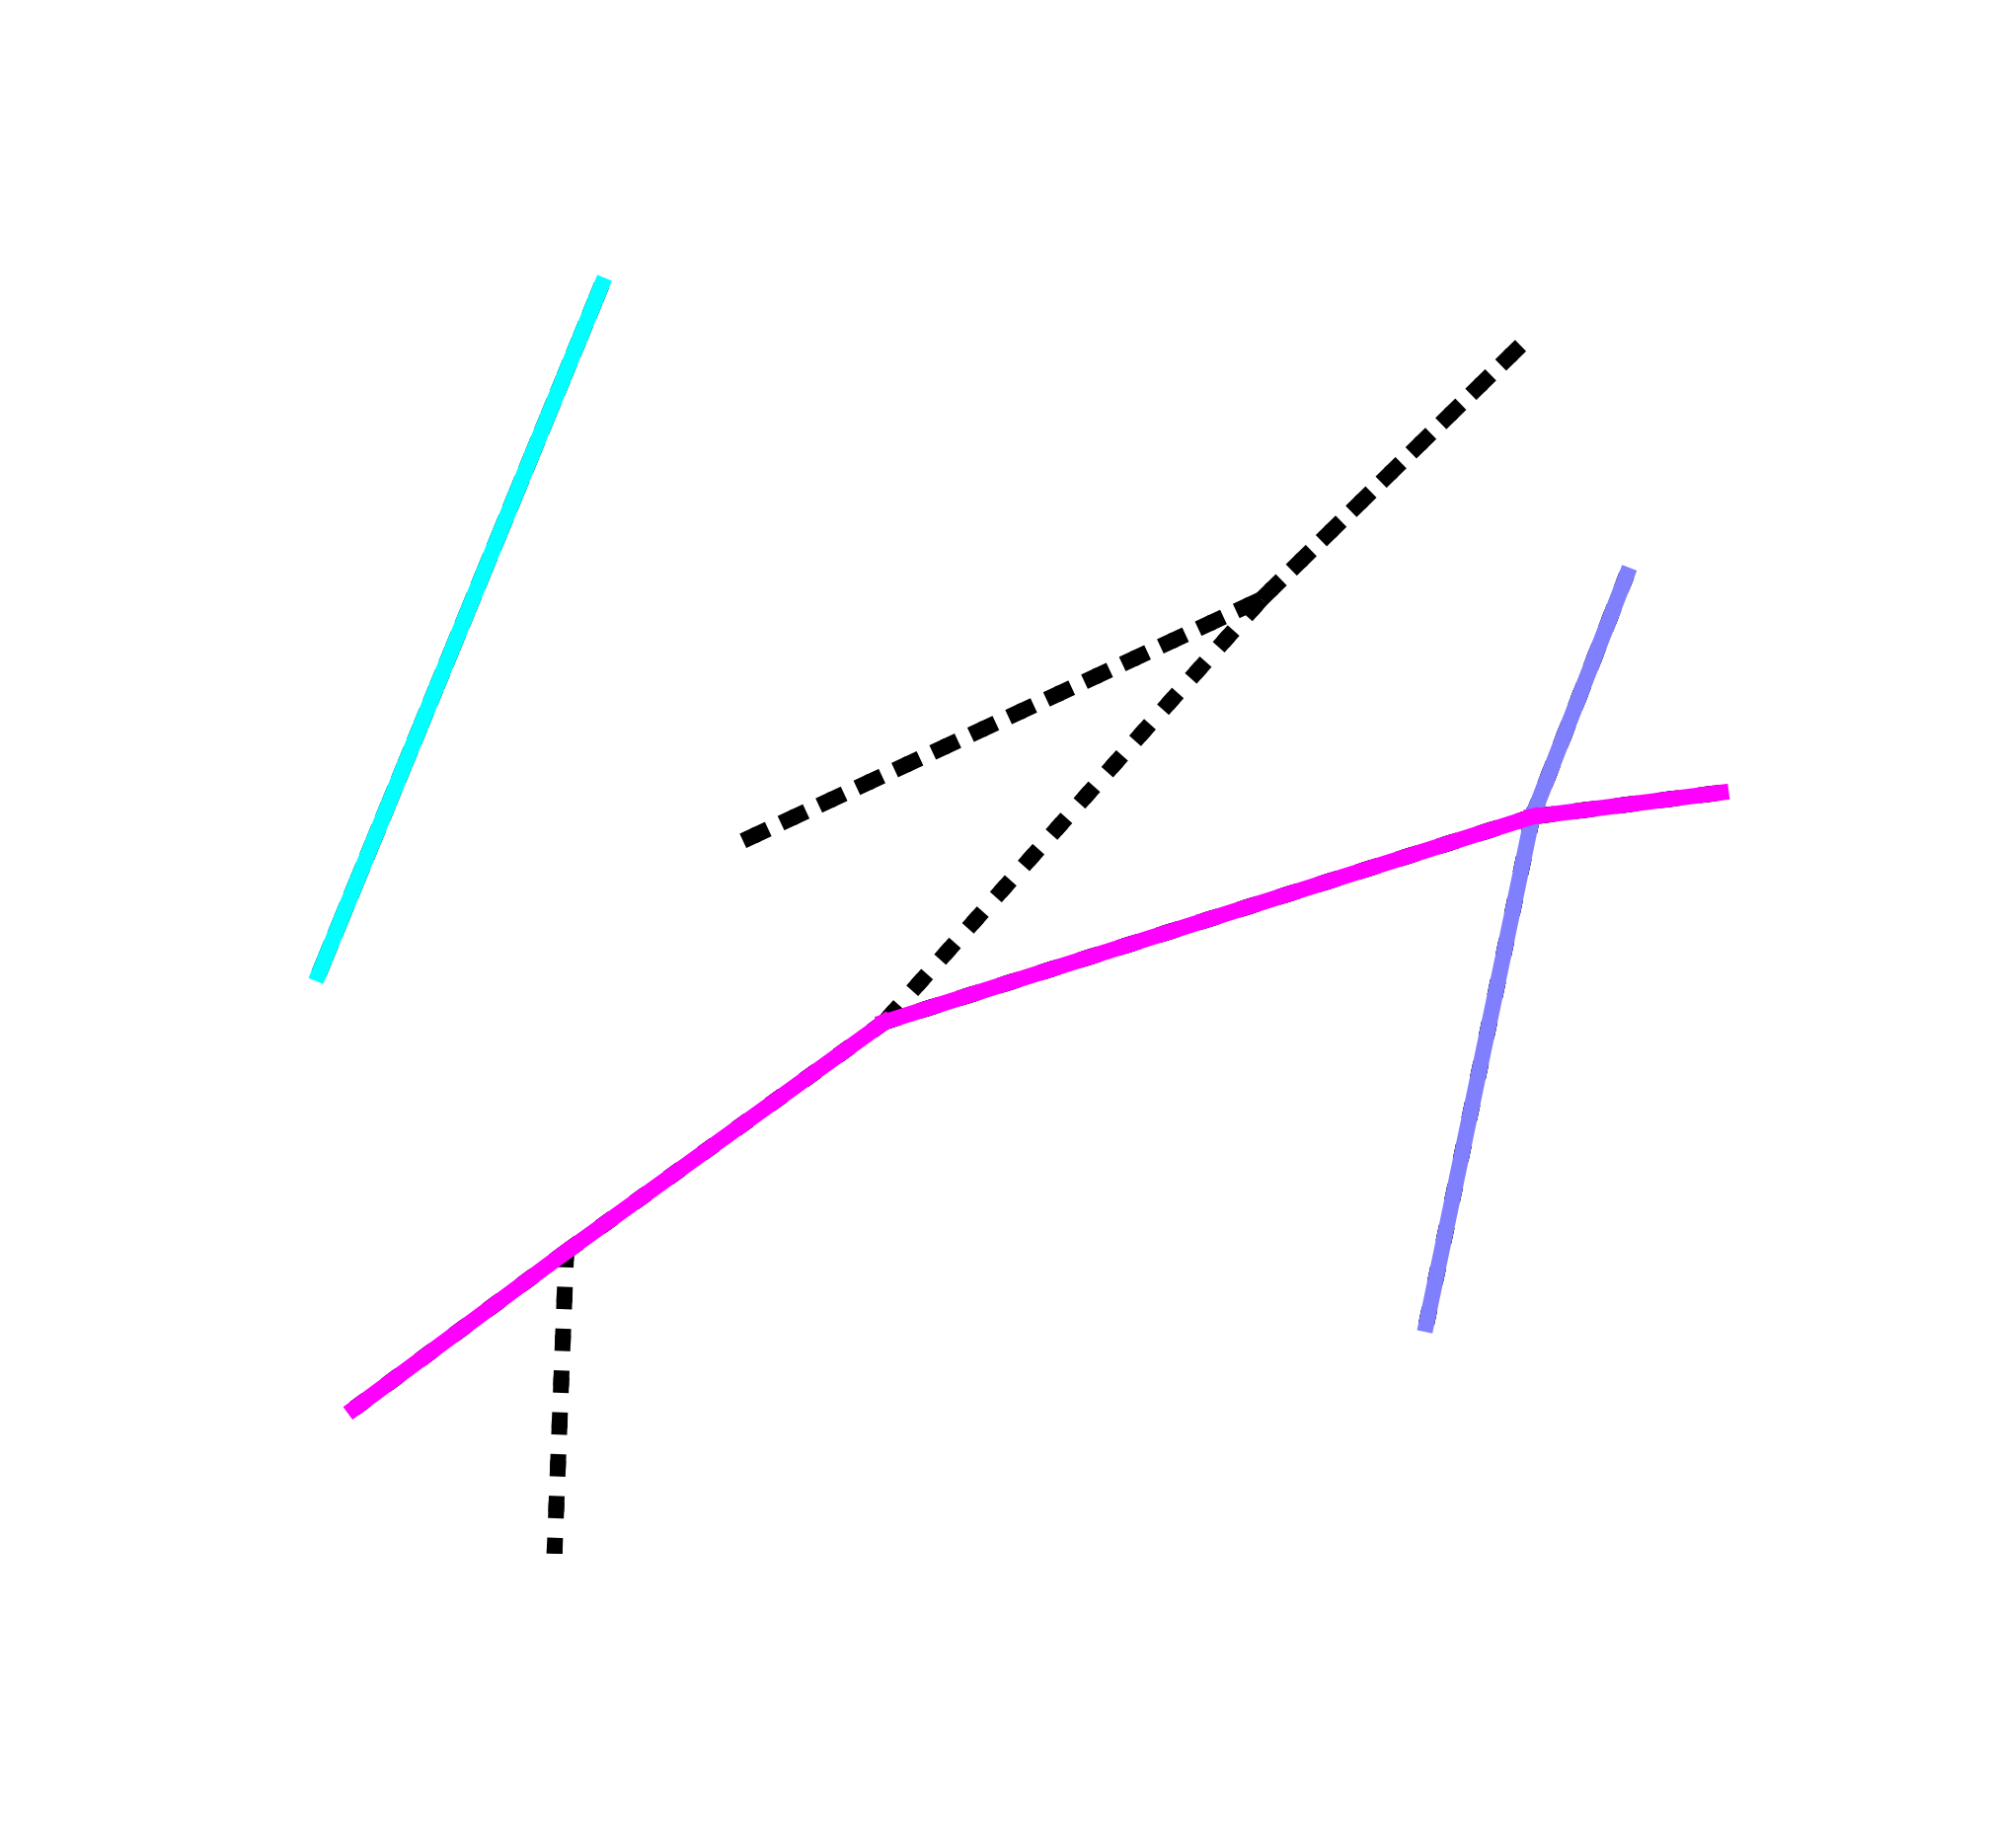
\includegraphics[scale=0.1]{resultImages/QFS7-DeFiNeExactMatch-60.png}
        \caption{3 filamentos correctamente individualizados por DeFiNe con 60\textdegree .}
        \label{fig:SpinningMarchantiaResults-define60Exact}
    \end{subfigure}
    \vskip\baselineskip
    
    \begin{subfigure}[t]{0.49\textwidth}
        \centering
        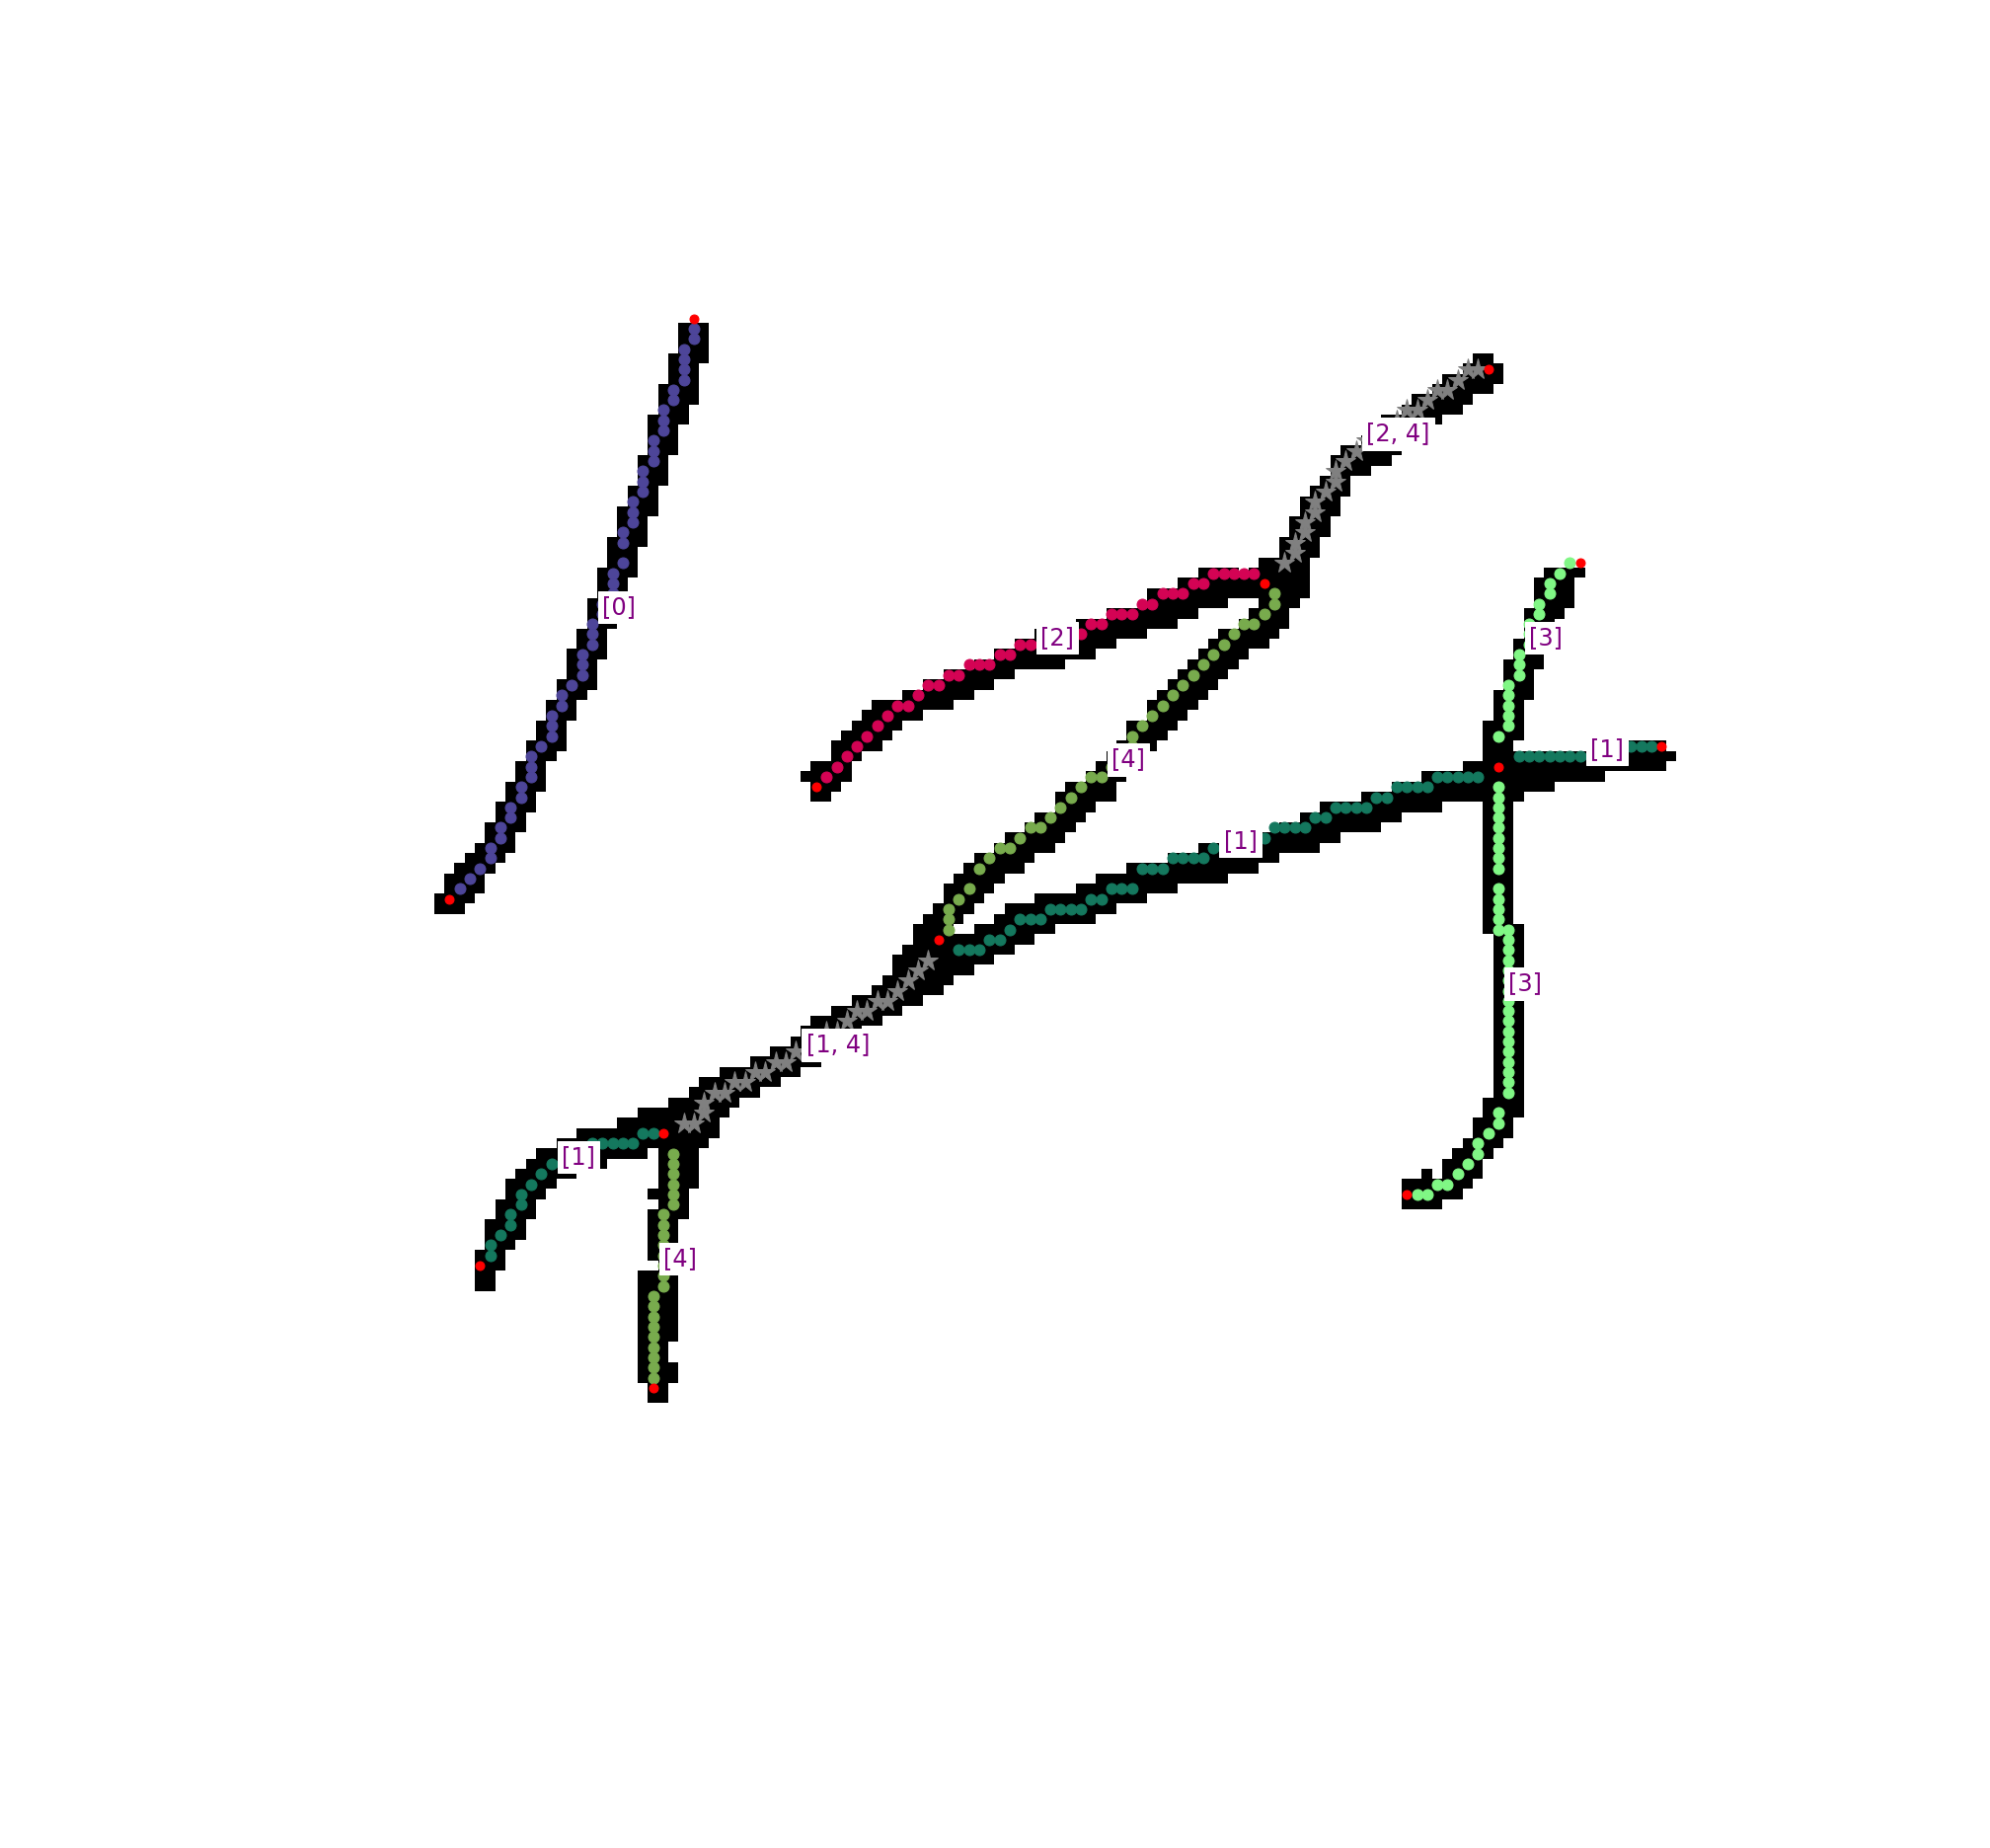
\includegraphics[scale=0.13]{resultImages/Synth-QuantitativeIFS-Fig7-phil-s1271-v05-antLabeled.png}
        \caption{Filamentos individualizados por la mejor iteraci\'on del algoritmo propuesto.}
        \label{fig:SynthQFS7-Individualizacion}
    \end{subfigure}
    ~
    \begin{subfigure}[t]{0.49\textwidth}
        \centering
        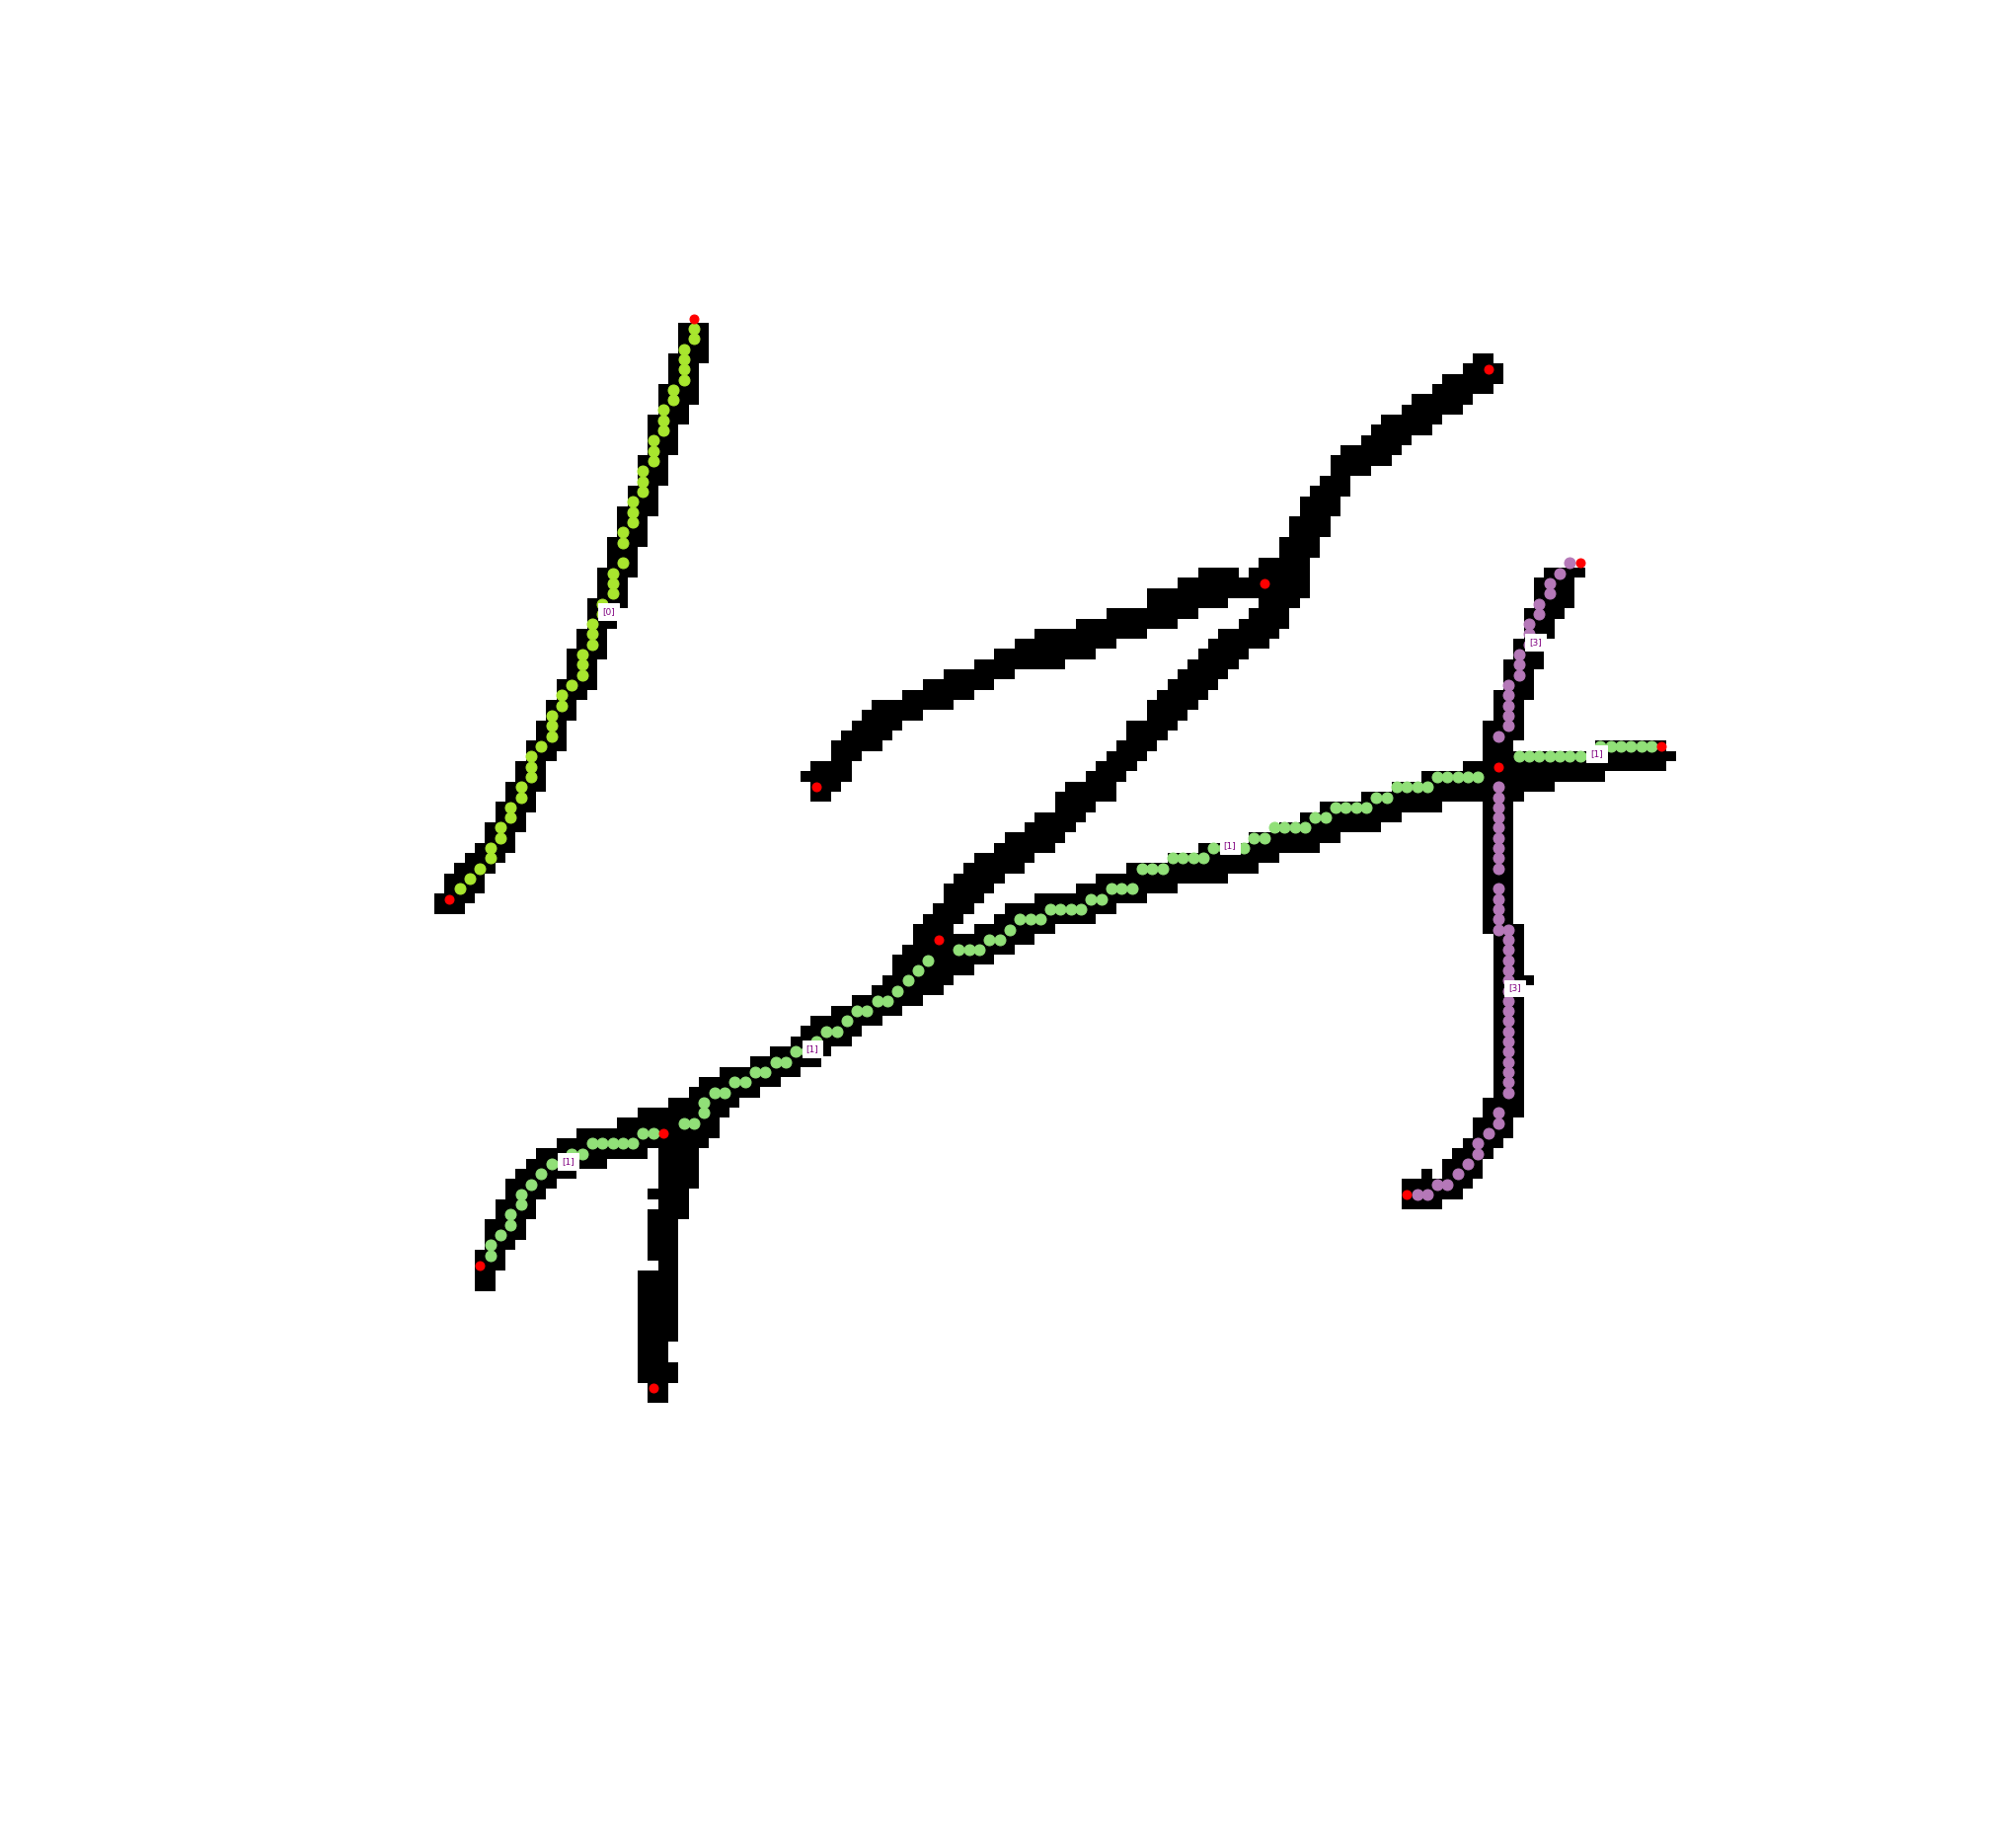
\includegraphics[scale=0.13]{resultImages/Synth-QuantitativeIFS-Fig7-phil-s1271-v05-exactMatch-antLabeled.png}
        \caption{3 filamentos correctamente individualizados  por la mejor iteraci\'on del algoritmo propuesto.}
        \label{fig:SynthQFS7-Individualizacion-Best}
    \end{subfigure}
    
    \caption{...}
    \label{fig:Synth-QIFS-Result}
\end{figure*}

\clearpage
\newpage
%%%%%%%%%% End synth QFS 7 - Begin Synth DeFiNe 1b %%%%%%%



%Resultados Synth Define

Como se menciona en la secci\'on \ref{sec:graphImageExtraction}, la Figura \ref{fig:synth-Define-1b} corresponde a una parte de la Figura 1b en \ref{fig:define-set-cover}, siendo la \'unica imagen para la que se dispone de un grafo ponderado seg\'un el criterio de los autores de DeFiNe. As\'i, se asume que aquel es el resultado \'optimo, en el que se individualizan correctamente los 5 filamentos. Una diferencia del grafo utilizado en la evaluaci\'on del algoritmo propuesto, con respecto al grafo que permite individualizar aquellos 5 filamentos, radica en que el utilizado con el algoritmo propuesto divide 1 de los 5 filamentos en 2, generando 6 filamentos en total. Es por ello, que las dem\'as evaluaciones con respecto a la Figura \ref{fig:synth-Define-1b} indican 6 filamentos como {\it ground truth}.


En la evaluaci\'on del algoritmo propuesto, se obtienen 3 individualizaciones correctas si se utilizan los par\'ametros definidos para microt\'ubulos de plantas. De estos 3 filamentos, uno corresponde a un filamento que no se encuentra aislado. Es posible atribuir esto a la curvatura de algunos de los filamentos sint\'eticos, la que es mayor a la que se espera de un microt\'ubulos de planta.


Con respecto a las medidas, se obtiene un alto valor de VI, lo que es atribuible a que en este caso existen varios casos de solapamiento entre filamentos, mientras que con la configuraci\'on para microt\'ubulos de planta, los \'indices {\it Rand} y {\it Jaccard} son disimiles entre s\'i, con enf\'asis en que el \'indice {\it Jaccard} arroja un resultado muy cercano a 0.


\begin{table}[h]
    \centering
    \begin{tabular}{|c|c|c|c|c|c|c|c|c|c|c|}
    \hline
        Algoritmo & VI & TP & FP &TN &FN & Rand	& Jaccard &	Precision &	Recall &	F1 \\ \hline
        Define 30° & 1.8102 & 6 & 14 & 156  & 34 & 0.7714 & 0.1111  & 0.3 & 0.15 & 0.2\\
        Define 60° & 2.2890 & 19 & 52 & 200 & 54 & 0.6738 & 0.152 & 0.2676  & 0.2602  & 0.2638\\ 
        Propuesta & 2.2164 & 22.8 & 40 & 240.4 & 61.4 & 0.7227 & 0.1838 & 0.3607 & 0.2724 & 0.3100\\
        \hline
    \end{tabular}
    \caption{Resultados de individualizaci\'on de filamentos para figura \ref{fig:synth-Define-1b}.El valor m\'aximo de VI en este caso es de 3.044522, ya que el tama\~no del {\it data set} es de 17 aristas. El n\'umero de filamentos en el {\it ground truth} es 5.}
    \label{tab:synth-Define-1b}
\end{table}
\addtocounter{table}{-1}
\begin{table}[h]
    \centering
    \begin{tabular}{|c|c|c|c|c|c|c|}
    \hline
         & \multirow{4}{2cm}{\centering \% Cobertura de Aristas} & \multirow{4}{2cm}{Filamentos Propuestos} & \multirow{4}{2cm}{Filamentos Correctos} & \multirow{4}{2.5cm}{\% Correctos vs Propuestos} & \multirow{4}{2.5cm}{\centering \% Correctos vs {\it Ground Truth}} & \multirow{4}{1.2cm}{\centering Tiempo [seg]} \\
         &  &  &  & & &  \\
        Algoritmo &  &  &  & & &  \\
        &  &  &  & & &  \\ \hline
        Define 30° & 100 & 11 & 2 & 18.1818 & 40 & 2.8275\\
        Define 60° & 100 & 7 & 2 & 28.5714 & 40 & 3.6597\\ 
        Propuesta & 100 & 9.2 & 3 & 32.6667 & 60 & 0.5071\\
        \hline
    \end{tabular}
    \caption{Resultados ({\it Continuaci\'on}) de individualizaci\'on de filamentos para figura \ref{fig:synth-Define-1b}. El n\'umero de filamentos en el {\it ground truth} es 5.}
    %\label{tab:synth-QFS-7-Results2}
\end{table}

\begin{figure*}[h!]
    \centering
    \begin{subfigure}[t]{0.49\textwidth}
        \centering
        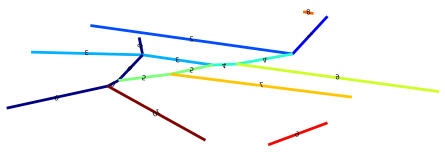
\includegraphics[scale=0.6]{resultImages/define-weighted-4-30.png}
        \caption{Individualizaci\'on mediante DeFiNe con 30\textdegree .}
        \label{fig:SynthDefine-Results-define30}
    \end{subfigure}%
    ~ 
    \begin{subfigure}[t]{0.49\textwidth}
        \centering
        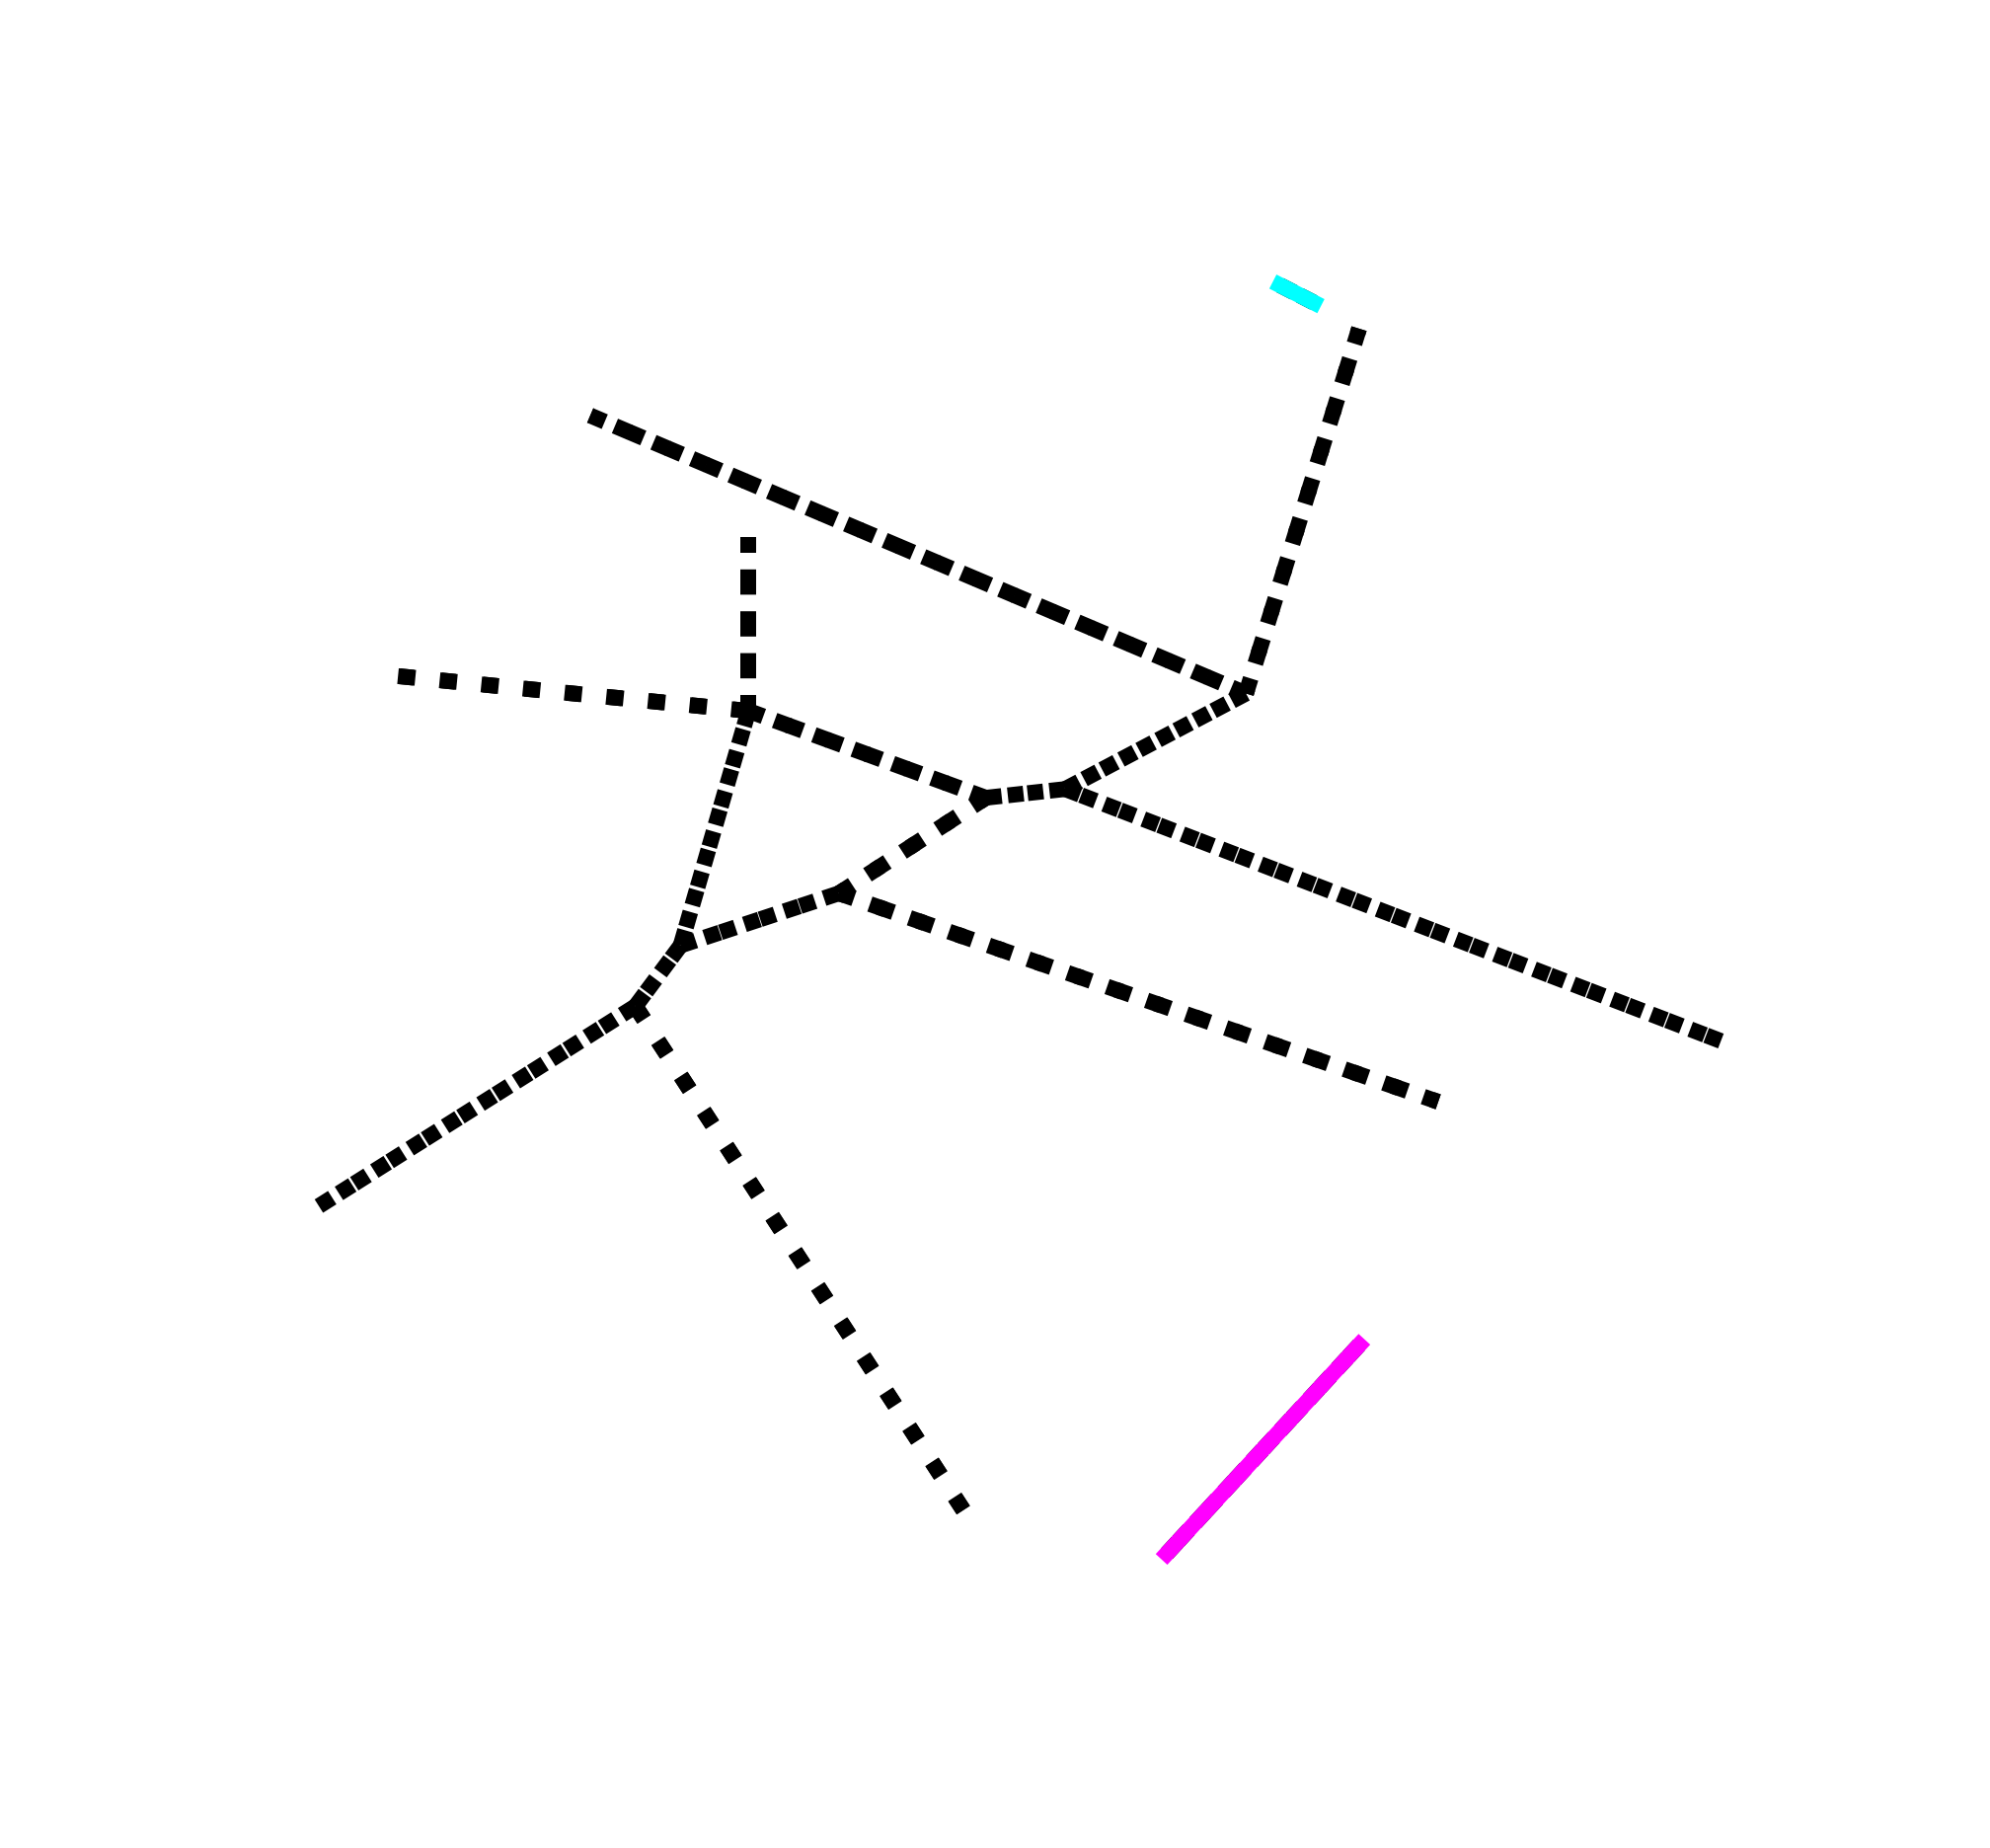
\includegraphics[height=1.5in]{resultImages/defineFig1b-DeFiNeExactMatch-30.png}
        \caption{3 filamentos correctamente individualizados por DeFiNe con 30\textdegree .}
        \label{fig:SynthDefine-Results-define30Exact}
    \end{subfigure}
    \vskip\baselineskip
    
    \begin{subfigure}[t]{0.49\textwidth}
        \centering
        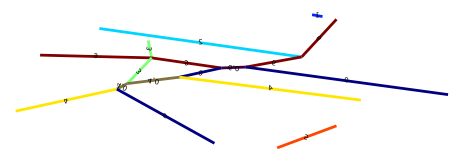
\includegraphics[scale=0.6]{resultImages/define-weighted-4-60.png}
        \caption{Individualizaci\'on mediante DeFiNe con 60\textdegree .}
        \label{fig:SynthDefine-Results-define60}
    \end{subfigure}
    ~ 
    \begin{subfigure}[t]{0.49\textwidth}
        \centering
        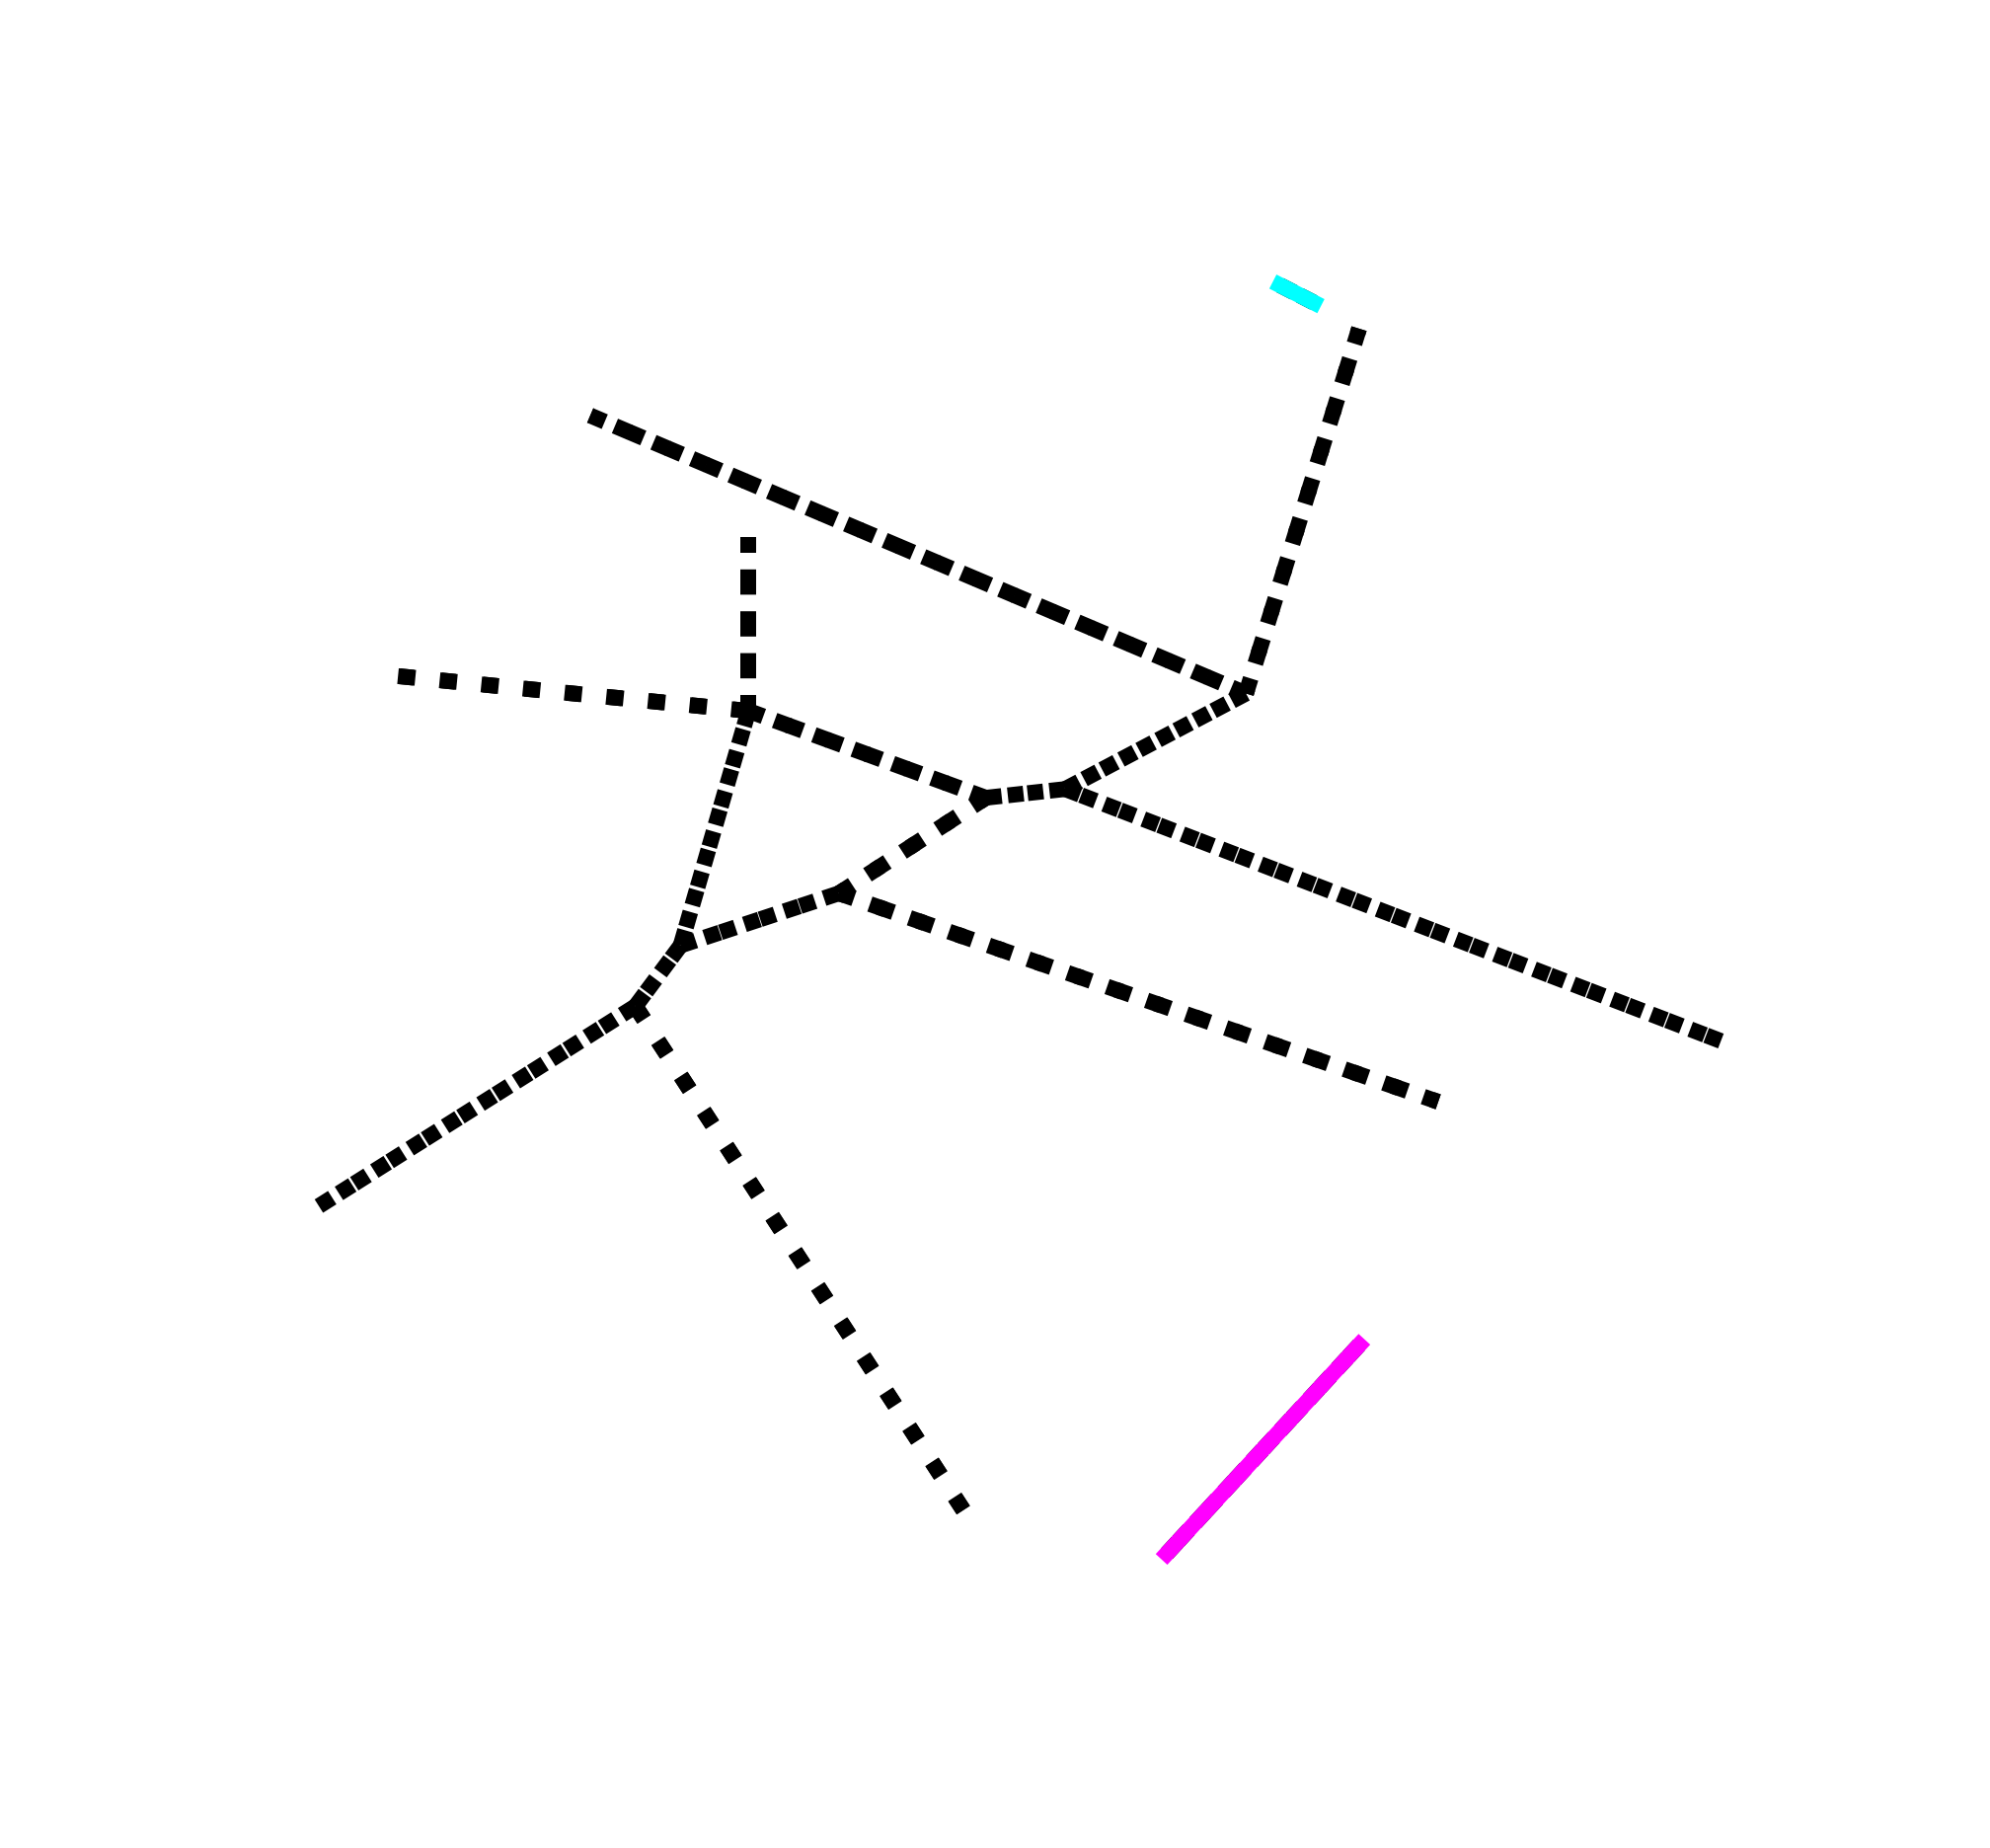
\includegraphics[scale=0.1]{resultImages/defineFig1b-DeFiNeExactMatch-60.png}
        \caption{4 filamentos correctamente individualizados por DeFiNe con 60\textdegree .}
        \label{fig:SynthDefine-Results-define60Exact}
    \end{subfigure}
    \vskip\baselineskip
    
    % \begin{subfigure}[t]{0.49\textwidth}
    %     \centering
    %     \includegraphics[scale=0.13]{}
    %     \caption{Filamentos individualizados por la mejor iteraci\'on del algoritmo propuesto.}
    %     \label{fig:SynthDefine-Individualizacion}
    % \end{subfigure}
    % ~
    % \begin{subfigure}[t]{0.49\textwidth}
    %     \centering
    %     \includegraphics[scale=0.13]{}
    %     \caption{3 filamentos correctamente individualizados  por la mejor iteraci\'on del algoritmo propuesto.}
    %     \label{fig:SynthDefine-Individualizacion-Best}
    % \end{subfigure}
    
    \caption{...}
    \label{fig:SynthDefine-Result}
\end{figure*}

\clearpage
\newpage
%%%%%%%%%% End Synth DeFiNe 1b %%%%%%%

\section{Im\'agenes Reales}

%recordar que define es base de BFS-Overlap-pairwise-total-
% recordarr que son 5 iteraciones y se estan promediando los resultados, conectar con la columna cobertura 
En esta secci\'on se muestran los resultados de la individualizaci\'on de filamentos para 2 tipos de c\'elulas, los microt\'ubulos existentes en la planta {\it Arabidpsis Marchantia}, y las dendritas en neuronas. Para cada tipo de c\'elulas existen 3 im\'agenes reales con las que se cuenta con la respectiva individualizaci\'on manual realizada por un experto.

De acuerdo a lo mencionado en la secci\'on \ref{sec:acoInit}, algunos p\'arametros del algoritmo propuesto var\'ian dependiendo del tipo de c\'elula, mientras que otros son fijos. Para la individualizaci\'on de filamentos realizada en im\'agenes reales, los par\'ametros se indican en la Tabla \ref{tab:AlgoParams}.

\begin{table}[h]
    \centering
    \begin{tabular}{|c|c|c|c|}
        \hline
        ${}^\text{C\'elula}{\mskip -5mu/\mskip -3mu}_\text{Par\'ametro}$ & $\theta$ & $Max\_Angle$ & $Max\_Axial\_Displacement$  \\ \hline
        {\it Arabidopsis Marchantia} & 30\textdegree & 90\textdegree & 1.5\\
        Neurona & 45\textdegree & 90\textdegree & 2\\\hline
    \end{tabular}
    \caption{Par\'ametros variables utilizados durante la individualizaci\'on de filamentos en im\'agenes reales.}
    \label{tab:AlgoParams}
\end{table}

\subsection{Microt\'ubulos de planta}

%Valor m\'ax de VI para \ref{tab:SpinningMarchantiaResults1} es 3.4965.
%N\'umero de filamentos en el {\it Ground Truth} de la figura SpinningMarchanria es 12.
%Define y Phil presentan una propuesta de filamento para el ....

\begin{table}[t]
    \centering
    \begin{tabular}{|c|c|c|c|c|c|c|c|c|c|c|}
    \hline
        Algoritmo & VI & TP & FP &TN &FN & Rand	& Jaccard &	Precision &	Recall &	F1 \\ \hline
        Define 30° & 0.9696 & 23 & 12 & 465 & 28 & 0.9242 & 0.3650 & 0.6571 & 0.4509  & 0.5348 \\ 
        Define 60° & 2.2870  & 15 & 38 & 523 & 54 & 0.8539 & 0.1401 & 0.2830 & 0.2173 & 0.2459\\
        Propuesta 1.8376 & 43 & 54 & 815 & 78 & 0.8666 & 0.2457 & 0.4432 & 0.3553 & 0.3944 \\
        \hline
    \end{tabular}
    \caption{Resultados de individualizaci\'on de filamentos para la muestra MT-A en la figura \ref{fig:SpinningMarchantia}. El valor m\'aximo de VI en este caso es de 3.4965, ya que el tama\~no del {\it data set} es de 29 aristas. El n\'umero de filamentos en el {\it ground truth} es 12.}
    \label{tab:SpinningMarchantiaResults1}
\end{table}
\addtocounter{table}{-1}
\begin{table}[h]
    \centering
    \begin{tabular}{|c|c|c|c|c|c|c|}
    \hline
         & \multirow{4}{2cm}{\centering \% Cobertura de Aristas} & \multirow{4}{2cm}{Filamentos Propuestos} & \multirow{4}{2cm}{Filamentos Correctos} & \multirow{4}{2.5cm}{\% Correctos vs Propuestos} & \multirow{4}{2.5cm}{\centering \% Correctos vs {\it Ground Truth}} & \multirow{4}{1.2cm}{\centering Tiempo [seg]} \\
         &  &  &  & & &  \\
        Algoritmo &  &  &  & & &  \\
        &  &  &  & & &  \\ \hline
        Define 30° & 100 & 16 & 9 & 56.25       & 75          & 4.1087 \\
        Define 60° & 100 & 12 & 5 & 41.6666 & 41.6666 & 5.9999 \\ 
        Propuesta 100 & 12 & 7 & 58.3333 & 58.3333 & 0.6558 \\
        \hline
    \end{tabular}
    \caption{Resultados ({\it Continuaci\'on}) de individualizaci\'on de filamentos para la muestra MT-A en la figura \ref{fig:SpinningMarchantia}. El n\'umero de filamentos en el {\it ground truth} es 12.}
    %\label{tab:SpinningMarchantiaResults2}
\end{table}


\begin{figure*}[h!]
    \centering
    \begin{subfigure}[t]{0.49\textwidth}
        \centering
        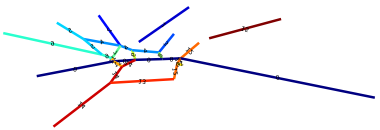
\includegraphics[scale=0.6]{resultImages/SpinningMarchantia-Define30.png}
        \caption{Individualizaci\'on mediante DeFiNe con 30\textdegree}
        \label{fig:SpinningMarchantiaResults-define30}
    \end{subfigure}%
    ~ 
    \begin{subfigure}[t]{0.49\textwidth}
        \centering
        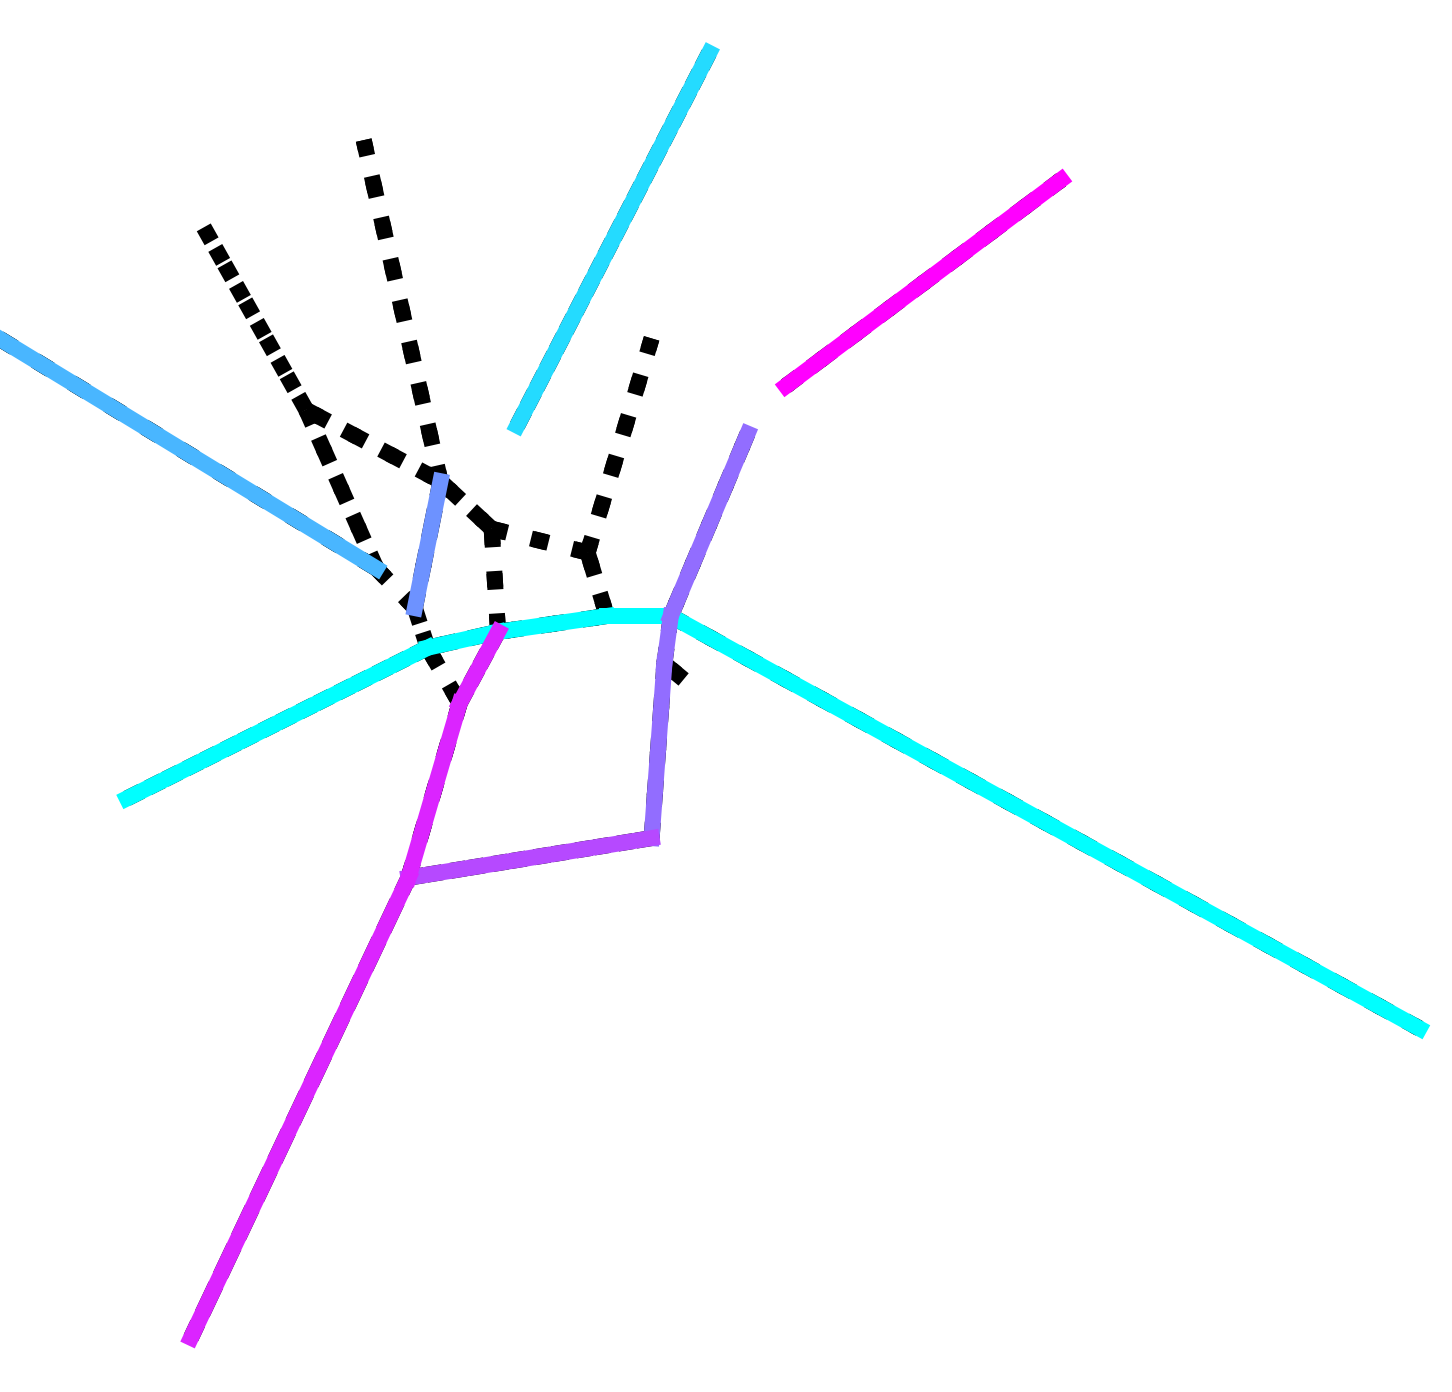
\includegraphics[height=1.5in]{resultImages/50-ROIs-Spinning-Marchantia-DeFiNeExactMatch-30.png}
        \caption{Filamentos correctamente individualizados por DeFiNe con 30\textdegree identificados con colores}
        \label{fig:SpinningMarchantiaResults-define30Exact}
    \end{subfigure}
    \vskip\baselineskip
    
    \begin{subfigure}[t]{0.49\textwidth}
        \centering
        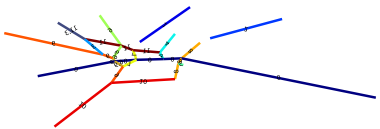
\includegraphics[scale=0.6]{resultImages/SpinningMarchantia-Define60.png}
        \caption{Individualizaci\'on mediante DeFiNe con 60\textdegree}
        \label{fig:SpinningMarchantiaResults-define60}
    \end{subfigure}
    ~ 
    \begin{subfigure}[t]{0.49\textwidth}
        \centering
        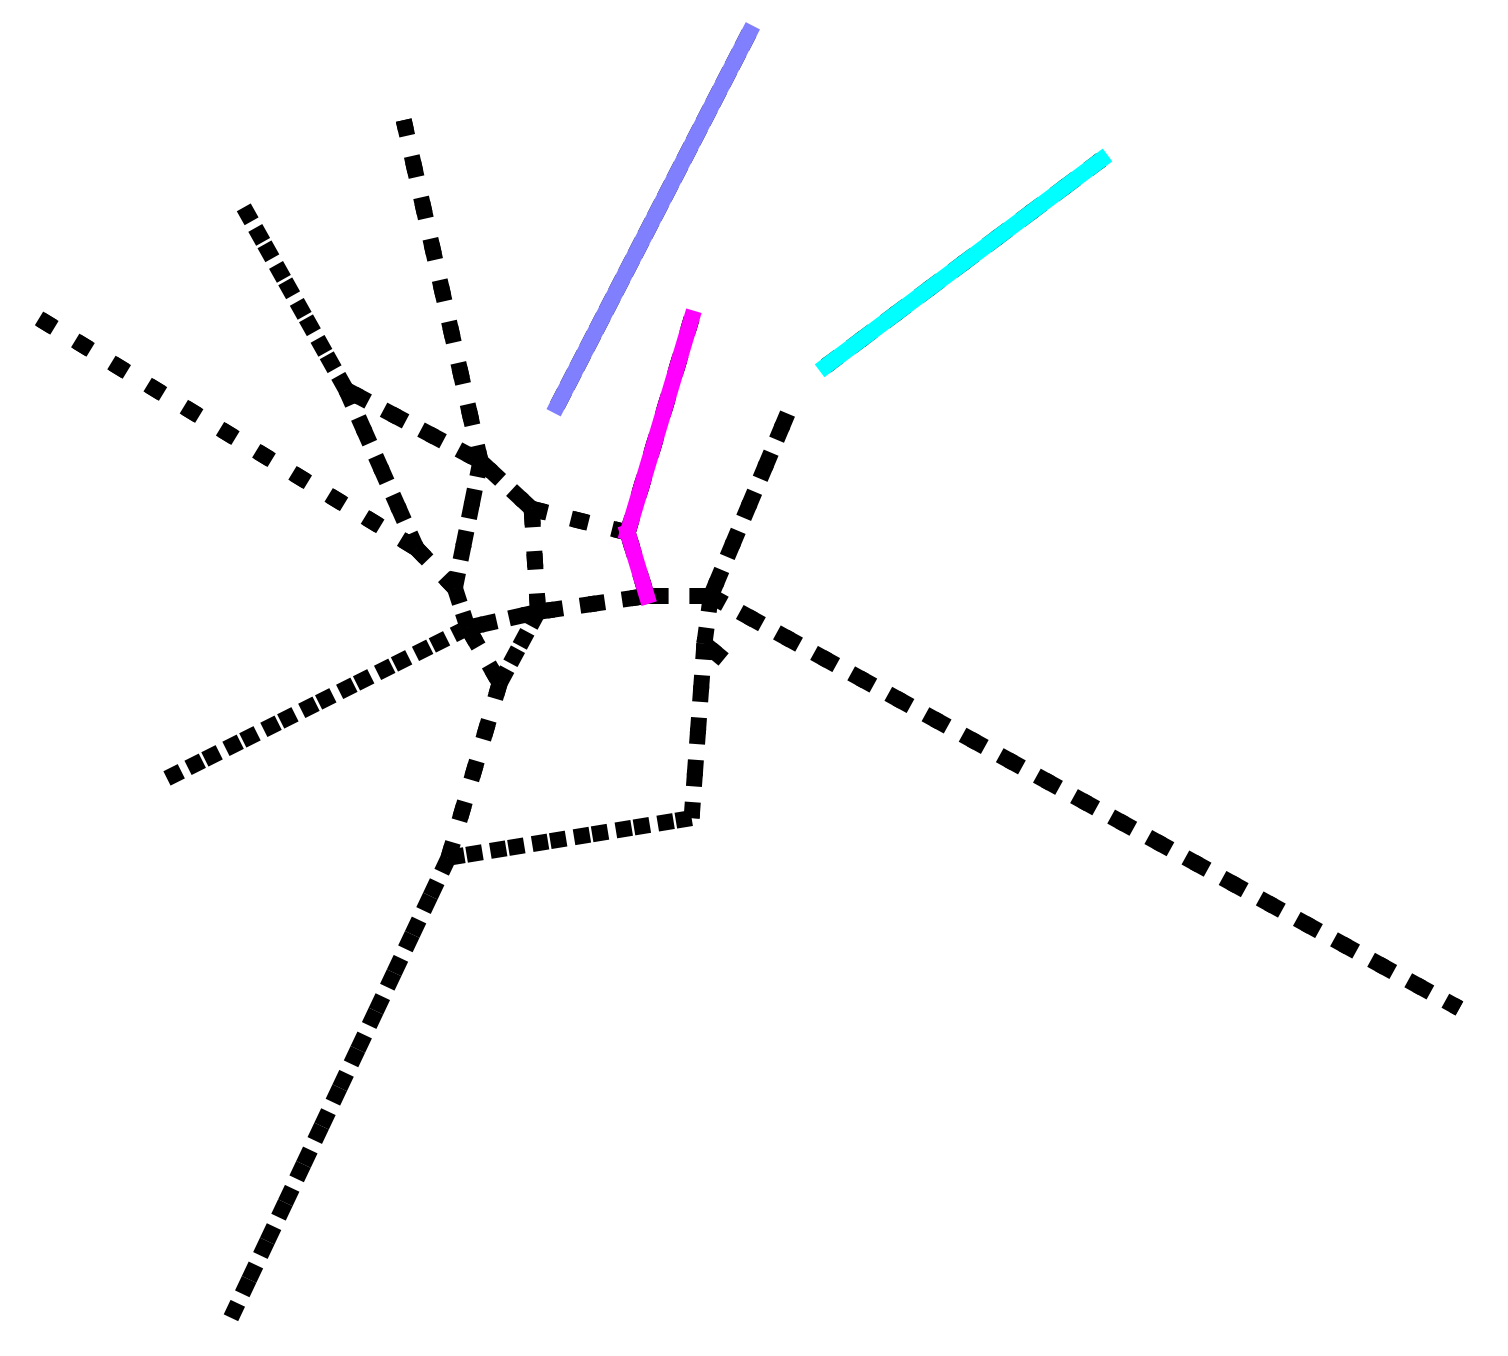
\includegraphics[height=1.5in]{resultImages/50-ROIs-Spinning-Marchantia-DeFiNeExactMatch-60.png}
        \caption{Filamentos correctamente individualizados por DeFiNe con 60\textdegree identificados con colores}
        \label{fig:SpinningMarchantiaResults-define60Exact}
    \end{subfigure}
    \vskip\baselineskip
    
    \begin{subfigure}[t]{0.49\textwidth}
        \centering
        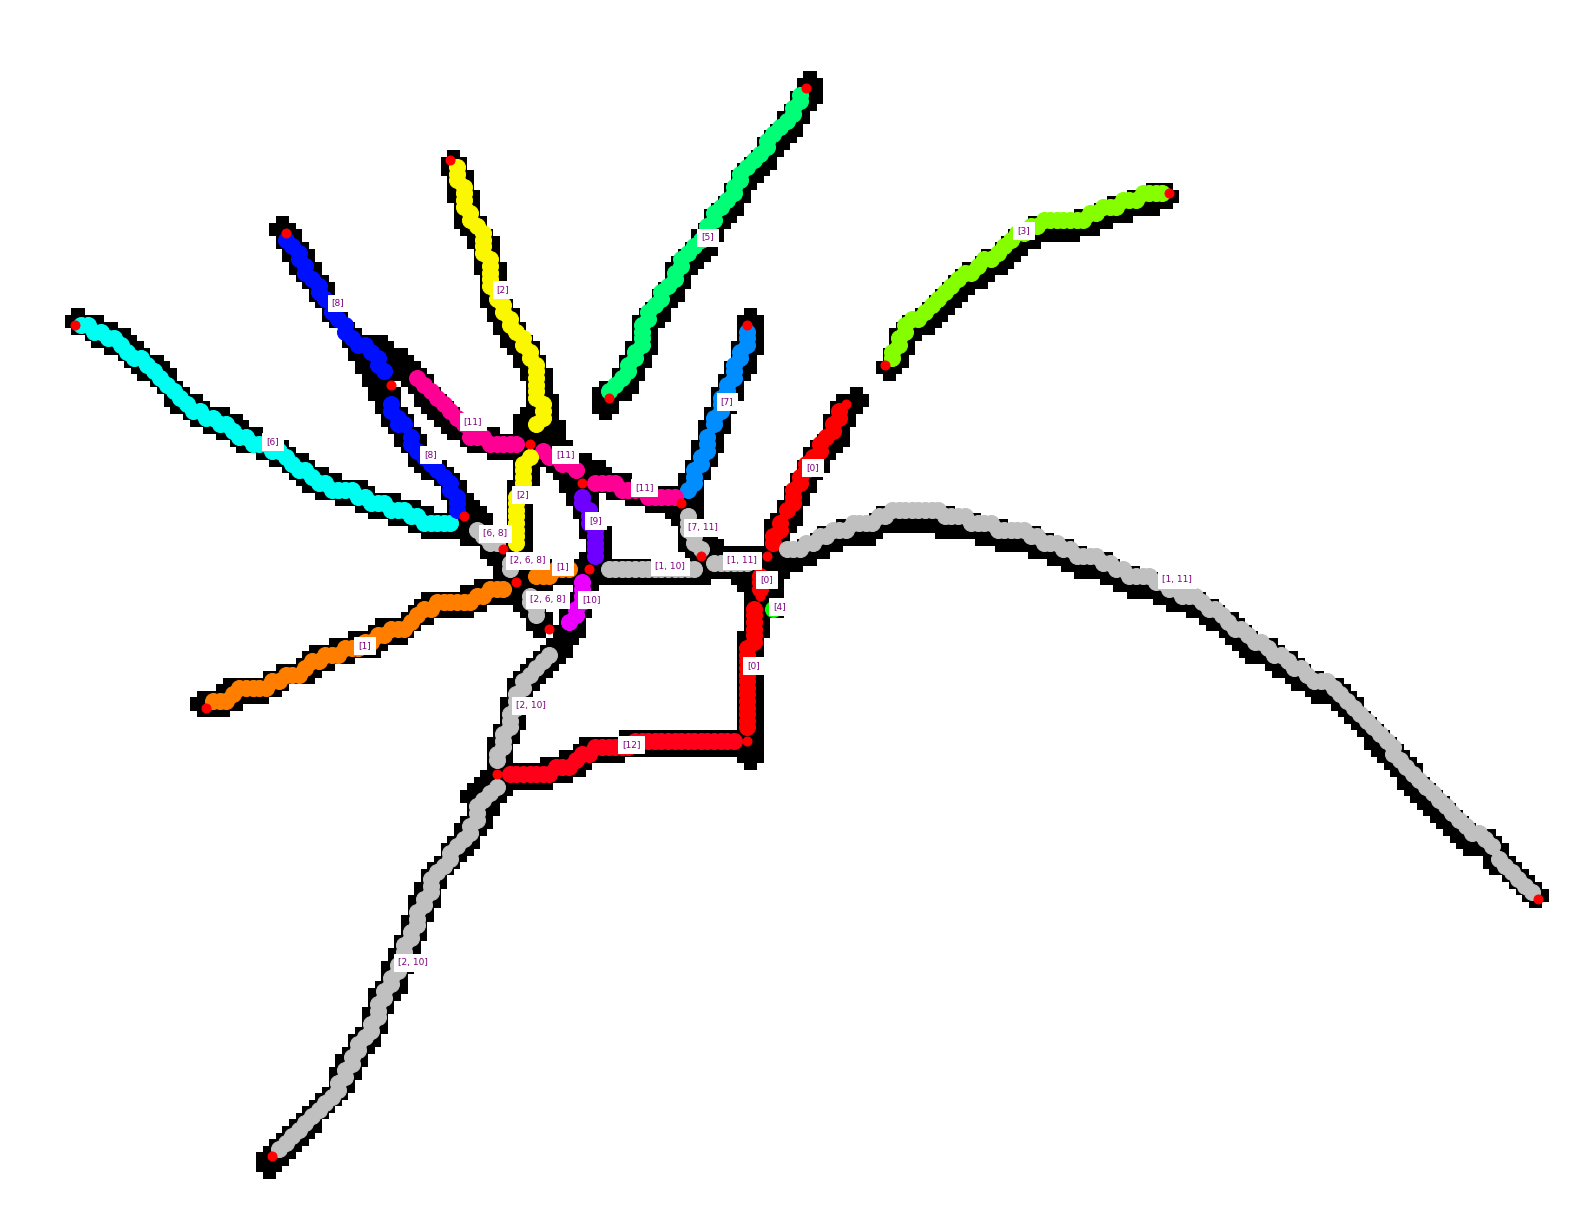
\includegraphics[height=1.5in]{resultImages/50-ROIs-Spinning-Marchantia-phil-s0-v05-antLabeled.png}
        \caption{Mejor resultado de individualizaci\'on de filamentos del algoritmo propuesto}
        \label{SpinningMarchantiaResults-bestPhil}
    \end{subfigure}
    ~
    \begin{subfigure}[t]{0.49\textwidth}
        \centering
        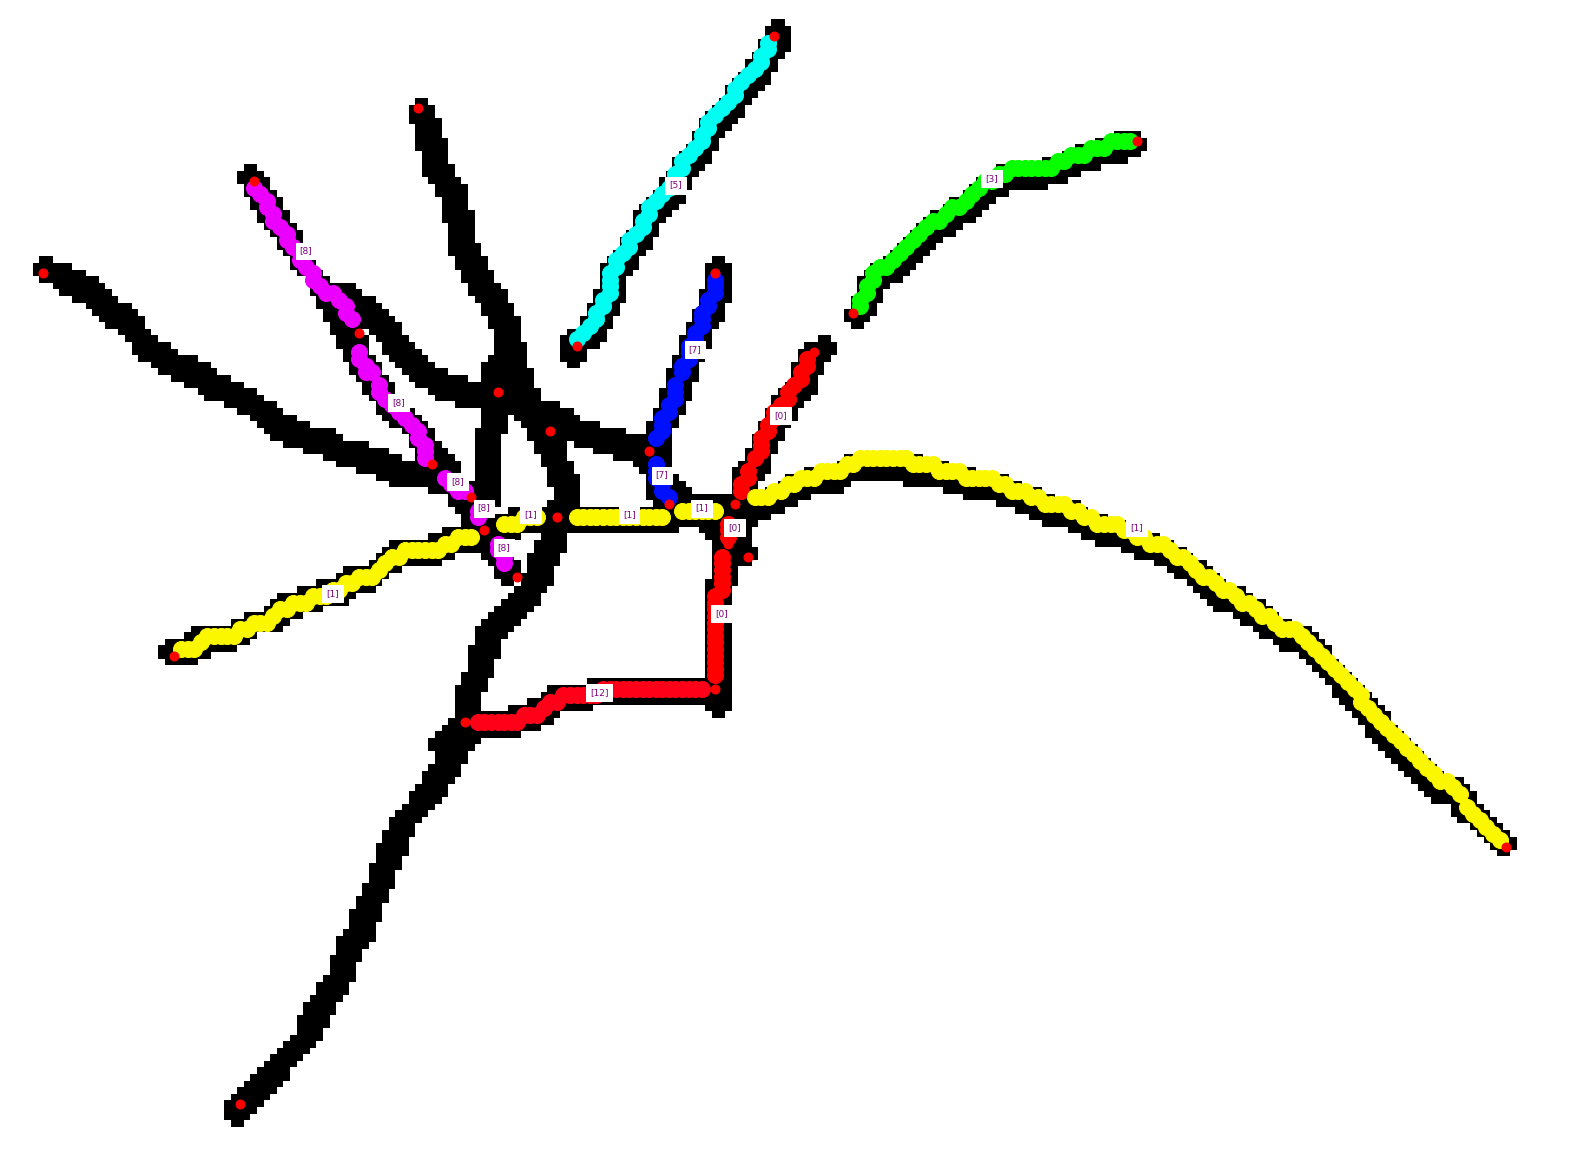
\includegraphics[height=1.5in]{resultImages/50-ROIs-Spinning-Marchantia-phil-s0-v05-exactMatch-antLabeled.png}
        \caption{Individualizaci\'on de filamentos correctos del mejor resultado del algoritmo propuesto}
        \label{fig:SpinningMarchantiaResults-bestPhilExact}
    \end{subfigure}
    \vskip\baselineskip
    
    \begin{subfigure}[t]{0.49\textwidth}
        \centering
        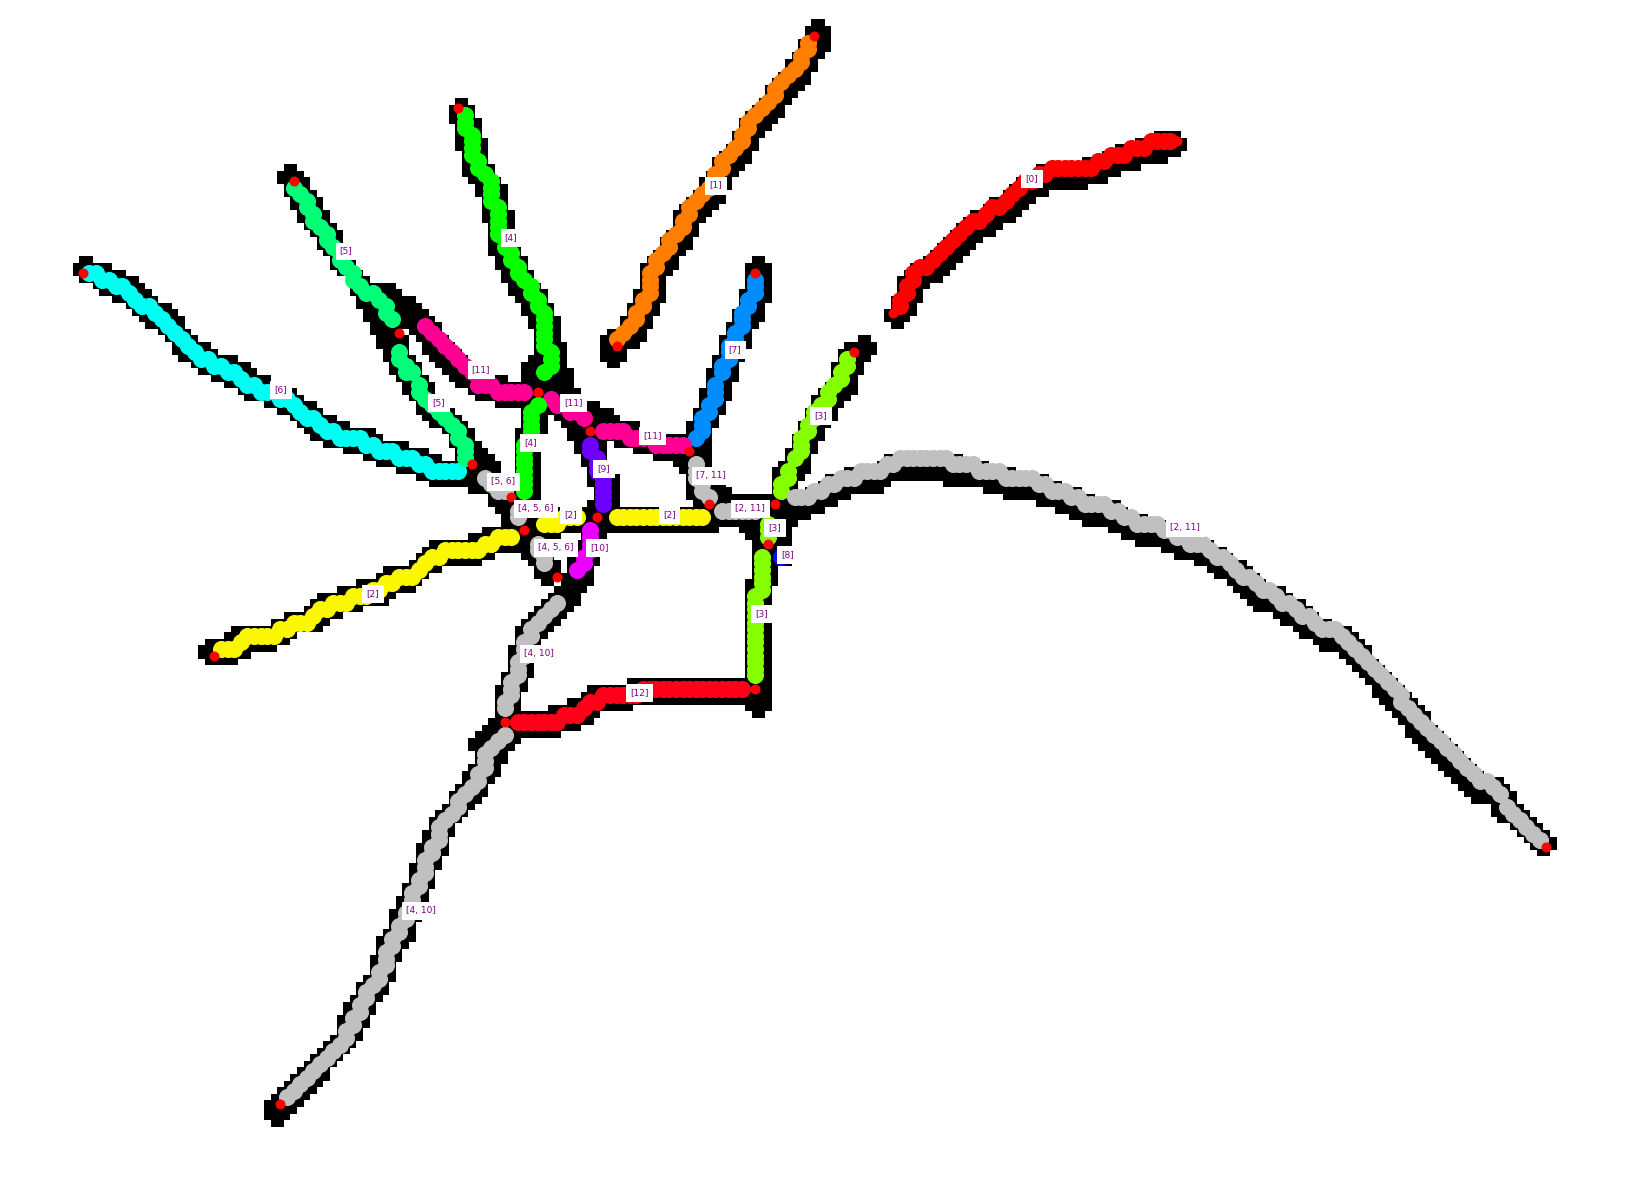
\includegraphics[height=1.5in]{resultImages/50-ROIs-Spinning-Marchantia-phil-s10-v05-antLabeled.png}
        \caption{Peor resultado de individualizaci\'on de filamentos del algoritmo propuesto}
        \label{SpinningMarchantiaResults-worstPhil}
    \end{subfigure}
    ~ 
    \begin{subfigure}[t]{0.49\textwidth}
        \centering
        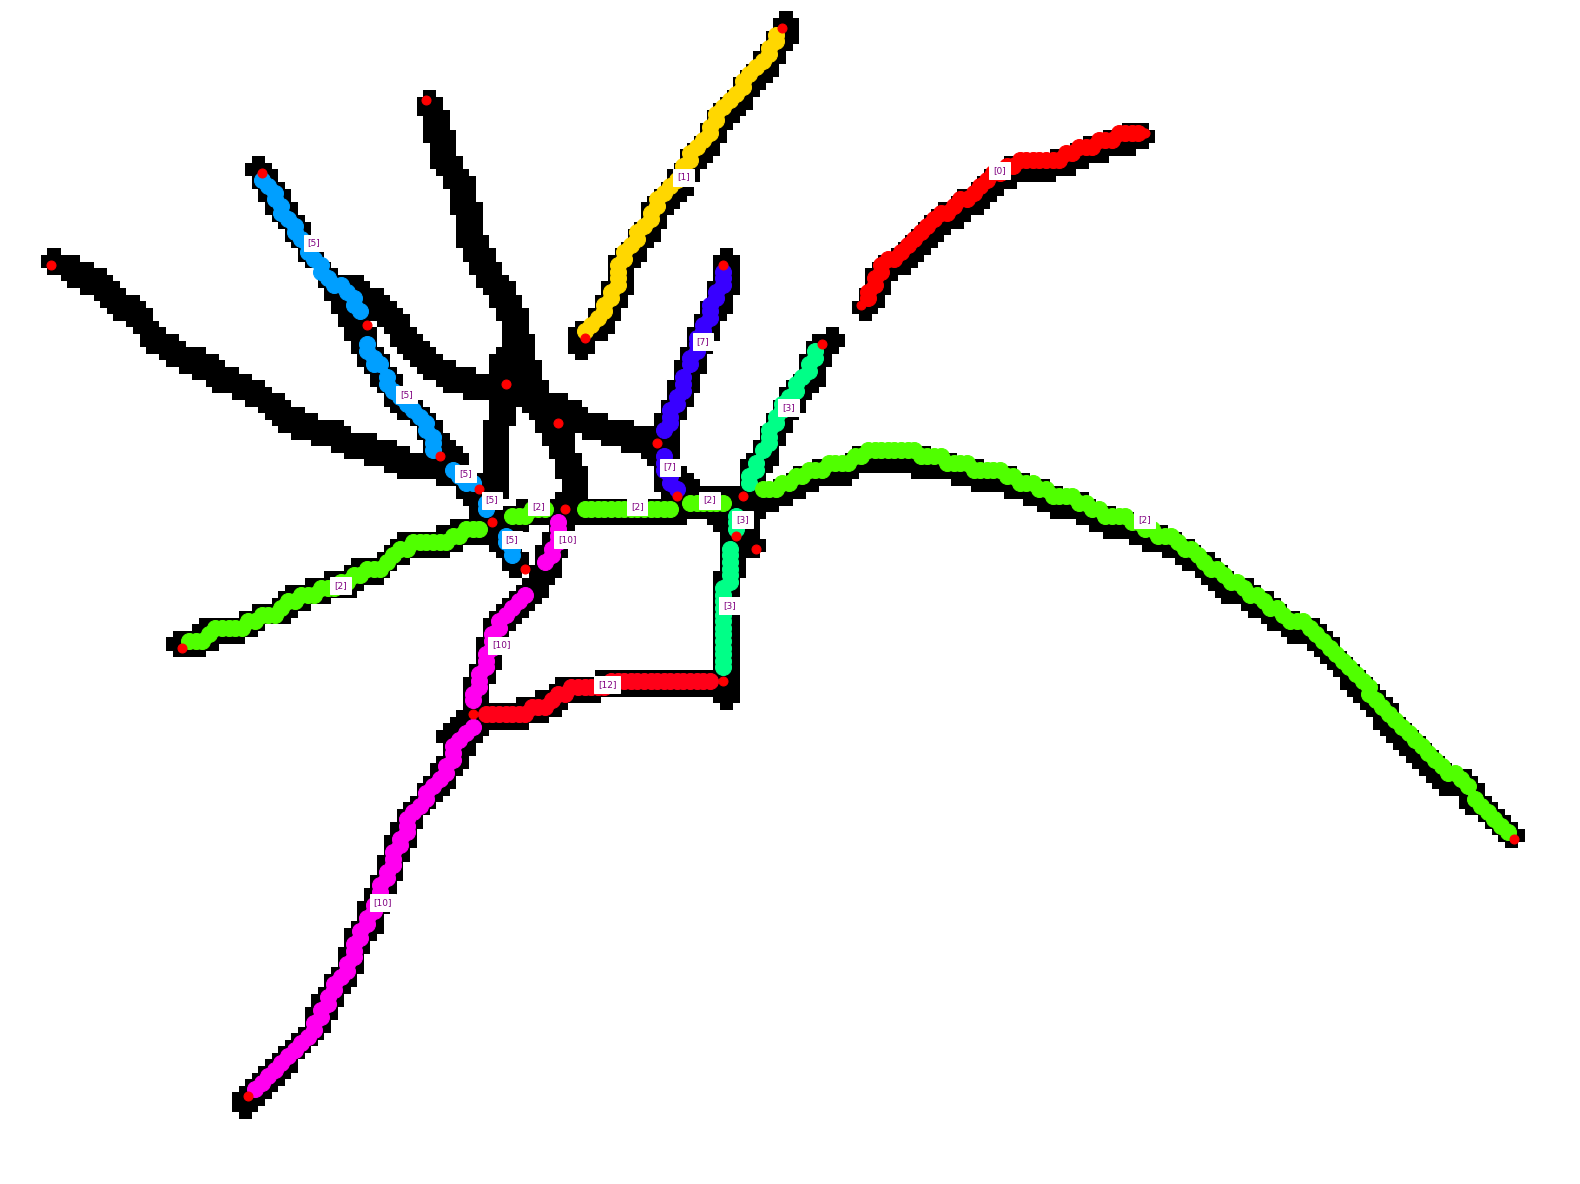
\includegraphics[height=1.5in]{resultImages/50-ROIs-Spinning-Marchantia-phil-s10-v05-exactMatch-antLabeled.png}
        \caption{Individualizaci\'on de filamentos correctos del peor resultado del algoritmo propuesto}
        \label{fig:SpinningMarchantiaResults-worstPhilExact}
    \end{subfigure}
    
    \caption{Individualizaci\'on  de filamentos para la muestra MT-A en la figura \ref{fig:SpinningMarchantia} realizadas con DeFiNe y Phil. Segmentos marcados en negro con y sin discontinuidad representan aristas no asignadas correctamente al filamento correspondiente en el {\it ground truth.}, mientras que los filamentos correctamente identificados se encuentran identificados mediante colores.}
    \label{fig:SpinningMarchantiaResults}
\end{figure*}

\clearpage
\newpage



%Valor m\'ax de VI para \ref{tab:field3t0filtered1} es 3.7612.
%N\'umero de filamentos en el {\it Ground Truth} de la figura field3t0 es 12.
para la muestra MT-B en la
- A pesar de tener el peor valor de VI, Phil obtiene la mayor cantidad de filamentos correctamente individualizados, en todos sus resultados. 
- encuentra el filamentos conformando por las aristas .... en 4 de las 5 iteraciones ejecutadas para obtener el comportamiento promedio. 
- El promedio de Phil tiene valores para TN/FP/TN/FN  mayores -> m\'as recorrido de soluciones?


\begin{table}[t]
    \centering
    \begin{tabular}{|c|c|c|c|c|c|c|c|c|c|c|}
    \hline
        Algoritmo & VI & TP & FP &TN &FN & Rand	& Jaccard &	Precision &	Recall &	F1 \\ \hline
        Define 30° & 1.9654 & 100 & 90 & 1615 & 148 & 0.8781 & 0.2958 & 0.5263 & 0.4032 & 0.4566\\
        Define 60° & 1.8847 & 18 & 17 & 962 & 84 & 0.9065 & 0.1512 & 0.5142 & 0.1764 & 0.2627\\ 
        Propuesta 2.3895 & 105.4 & 102.4 & 2028.4 & 224 & 0.8683 & 0.2487 & 0.5079 & 0.3283 & 0.3976 \\
        \hline
    \end{tabular}
    \caption{Resultados de individualizaci\'on de filamentos para la muestra MT-B (figura \ref{fig:field3t0filtered1}). El valor m\'aximo de VI en este caso es de 3.7612, ya que el tama\~no del {\it data set} es de 40 aristas. El n\'umero de filamentos en el {\it ground truth} es 12.}
    \label{tab:field3t0filtered1}
\end{table}
\addtocounter{table}{-1}
\begin{table}[h]
    \centering
    \begin{tabular}{|c|c|c|c|c|c|c|}
    \hline
         & \multirow{4}{2cm}{\centering \% Cobertura de Aristas} & \multirow{4}{2cm}{Filamentos Propuestos} & \multirow{4}{2cm}{Filamentos Correctos} & \multirow{4}{2.5cm}{\% Correctos vs Propuestos} & \multirow{4}{2.5cm}{\centering \% Correctos vs {\it Ground Truth}} & \multirow{4}{1.2cm}{\centering Tiempo [seg]} \\
         &  &  &  & & &  \\
        Algoritmo &  &  &  & & &  \\
        &  &  &  & & &  \\ \hline
        Define 30° & 100 & 23 & 5 & 21.7391 & 41.6667 & 5.0306 \\
        Define 60° & 100 & 16 & 5 & 31.25 & 41.6667 & 16.2042 \\ 
        Propuesta 100 & 15 & 8.8 & 58.7738 & 73.3333 & 0.9693 \\
        \hline
    \end{tabular}
    \caption{Resultados ({\it Continuaci\'on}) de individualizaci\'on de filamentos para la muestra MT-B (figura \ref{fig:field3t0filtered1}). El n\'umero de filamentos en el {\it ground truth} es 12.}
    %\label{tab:field3t0filtered1-2}
\end{table}


\begin{figure*}[h!]
    \centering
    \begin{subfigure}[t]{0.49\textwidth}
        \centering
        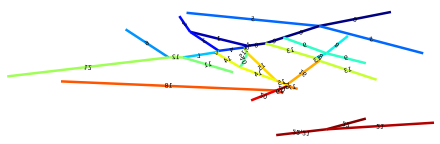
\includegraphics[scale=0.6]{resultImages/field3-t0-2cellBcrop-filtered-Define30.png}
        \caption{Individualizaci\'on mediante DeFiNe con 30\textdegree}
        \label{fig:field3t0filtered1Results-define30}
    \end{subfigure}%
    ~
    \begin{subfigure}[t]{0.49\textwidth}
        \centering
        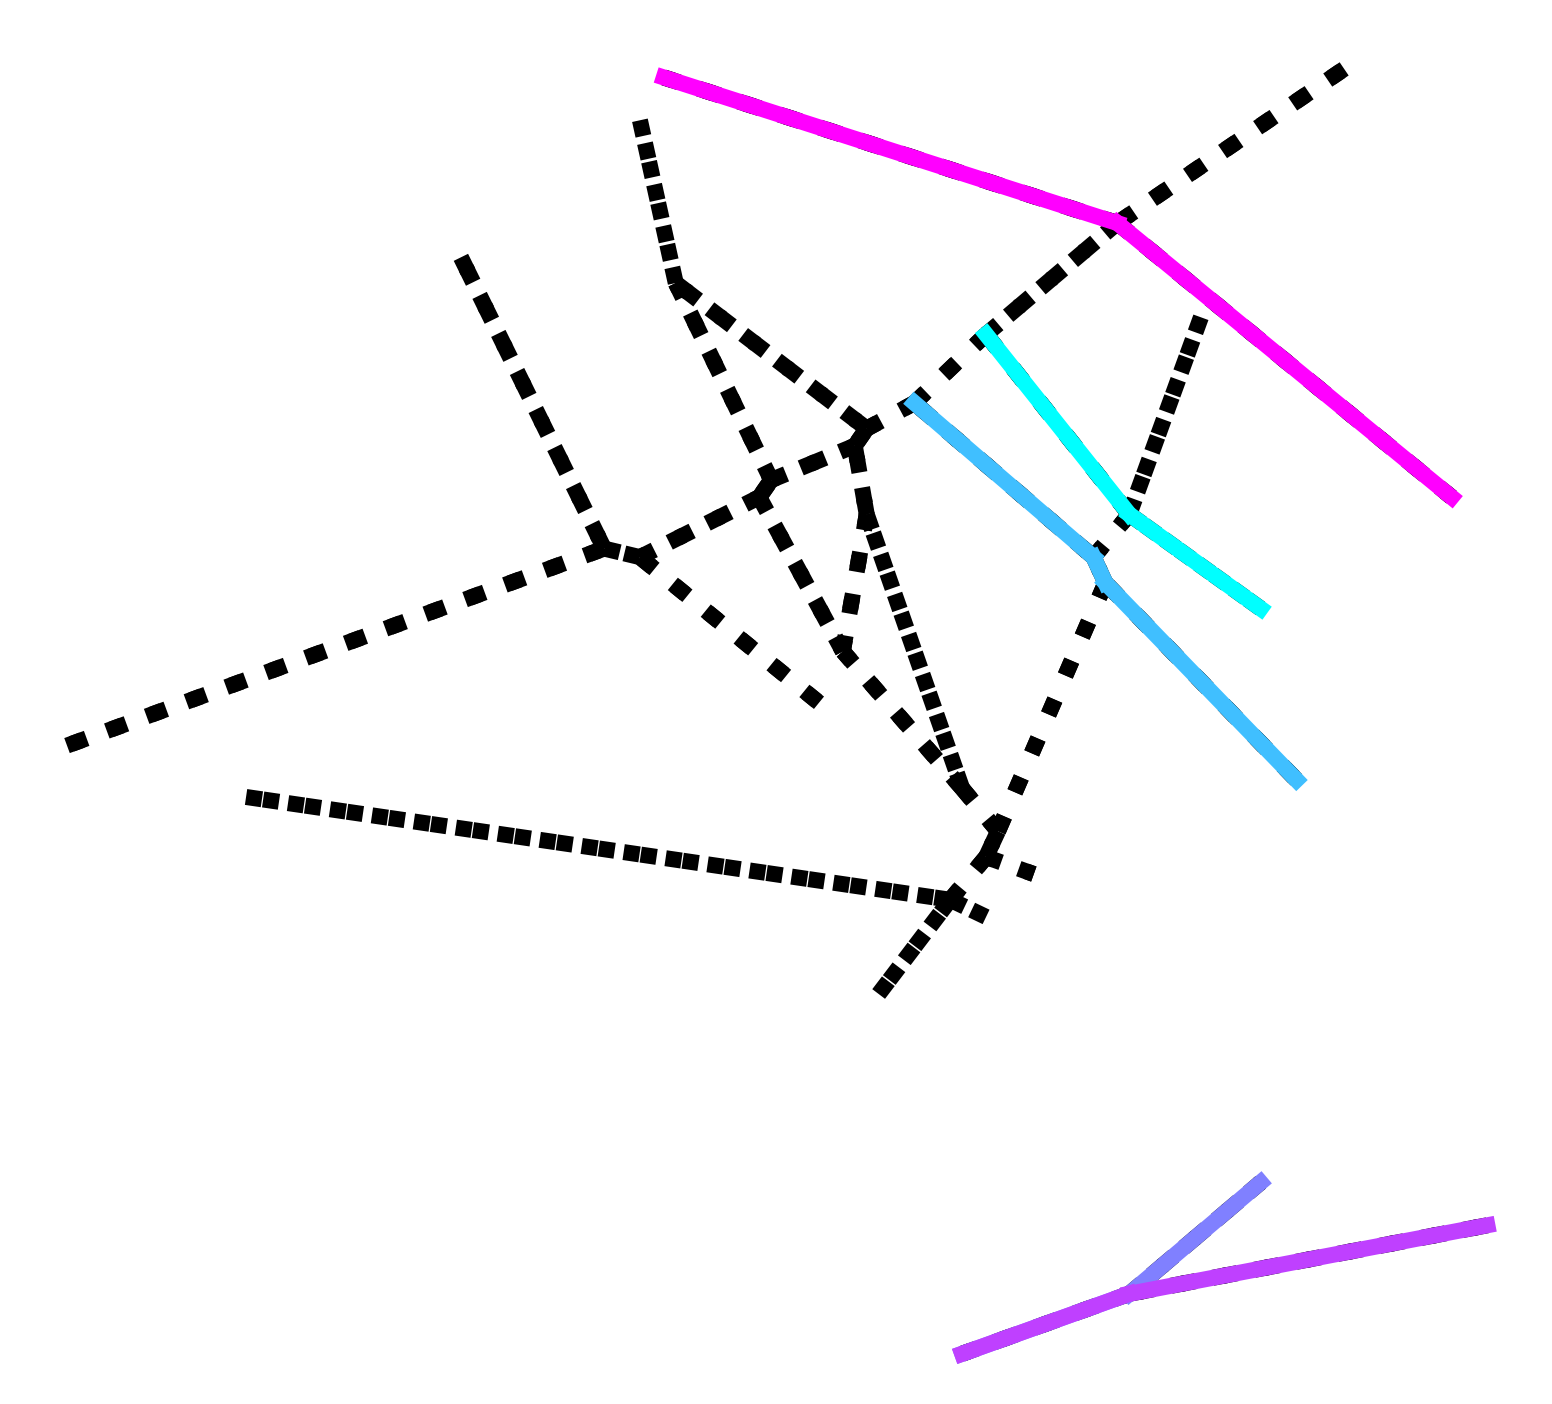
\includegraphics[height=1.5in]{resultImages/field3-t0-2cellBcrop-filtered-DeFiNeExactMatch-30.png}
        \caption{Filamentos correctamente individualizados por DeFiNe con 30\textdegree identificados con colores}
        \label{fig:field3t0filtered1Results-define30Exact}
    \end{subfigure}
    \vskip\baselineskip
    
    \begin{subfigure}[t]{0.49\textwidth}
        \centering
        \includegraphics[scale=0.6]{resultImages/field3-t0-2cellBcrop-filtered-DeFiNe60.png}
        \caption{Individualizaci\'on mediante DeFiNe con 60\textdegree}
        \label{fig:field3t0filtered1Results-define60}
    \end{subfigure}
    ~ 
    \begin{subfigure}[t]{0.49\textwidth}
        \centering
        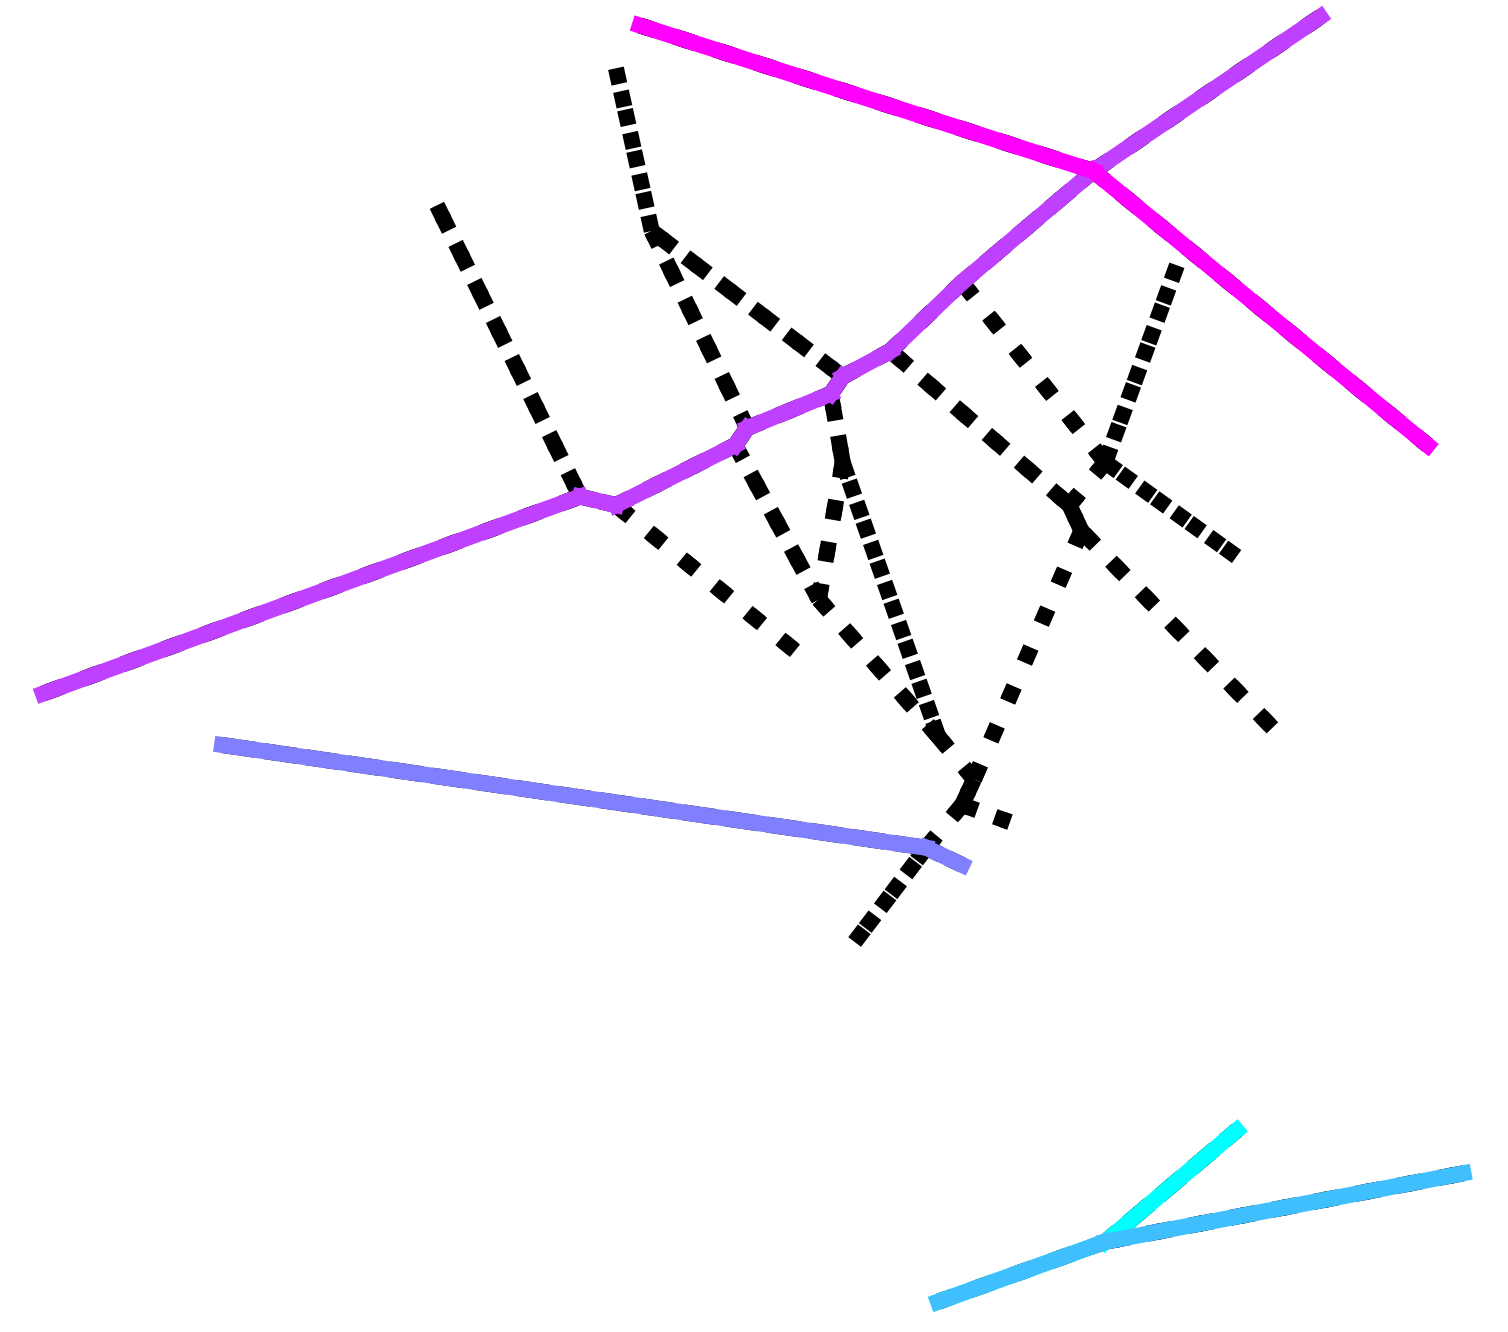
\includegraphics[height=1.5in]{resultImages/field3-t0-2cellBcrop-filtered-DeFiNeExactMatch-60.png}
        \caption{Filamentos correctamente individualizados por DeFiNe con 60\textdegree identificados con colores}
        \label{fig:field3t0filtered1Results-define60Exact}
    \end{subfigure}
    
    \vskip\baselineskip
    \begin{subfigure}[t]{0.49\textwidth}
        \centering
        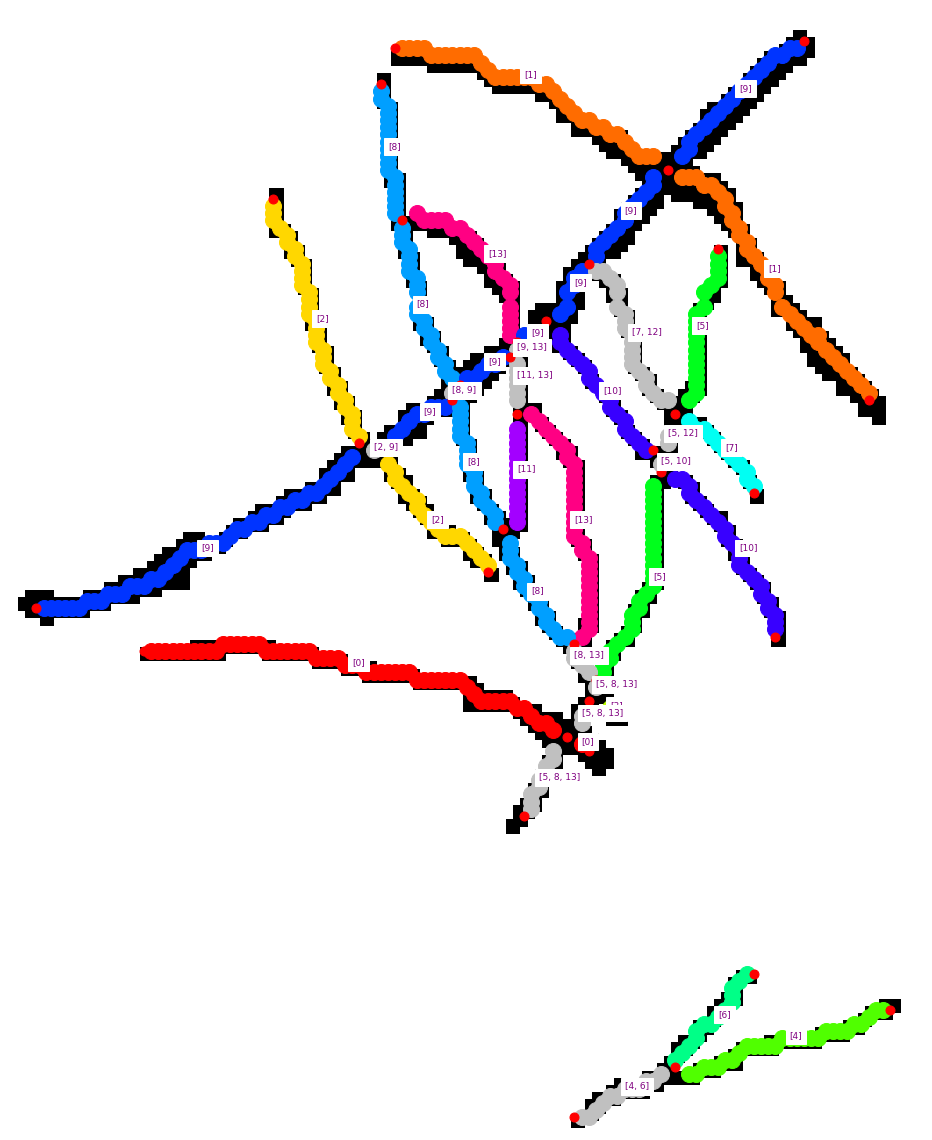
\includegraphics[height=1.5in]{resultImages/field3-t0-2cellBcrop-filtered-phil-s0-v05-antLabeled.png}
        \caption{Mejor Resultado de Individualizaci\'on con Phil}
        \label{field3t0filtered1Results-bestPhil}
    \end{subfigure}
    ~ 
    \begin{subfigure}[t]{0.49\textwidth}
        \centering
        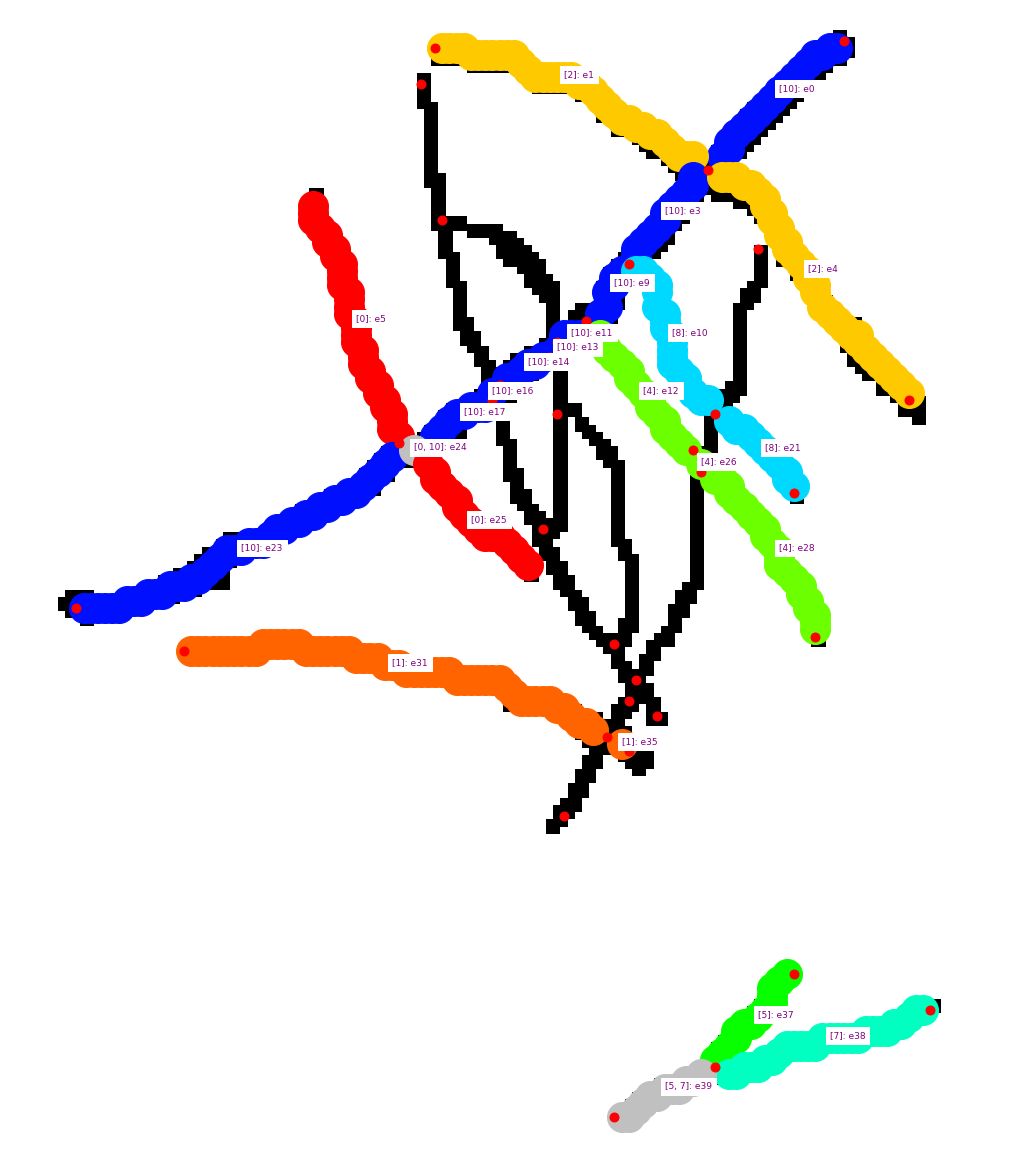
\includegraphics[height=1.5in]{resultImages/field3-t0-2cellBcrop-filtered-phil-s0-v05-exactMatch-antLabeled.png}
        \caption{Filamentos correctamente individualizados a partir del mejor resultado con Phil, identificados con colores}
        \label{fig:field3t0filtered1Results-bestPhilExact}
    \end{subfigure}
    \vskip\baselineskip
    
    \begin{subfigure}[t]{0.49\textwidth}
        \centering
        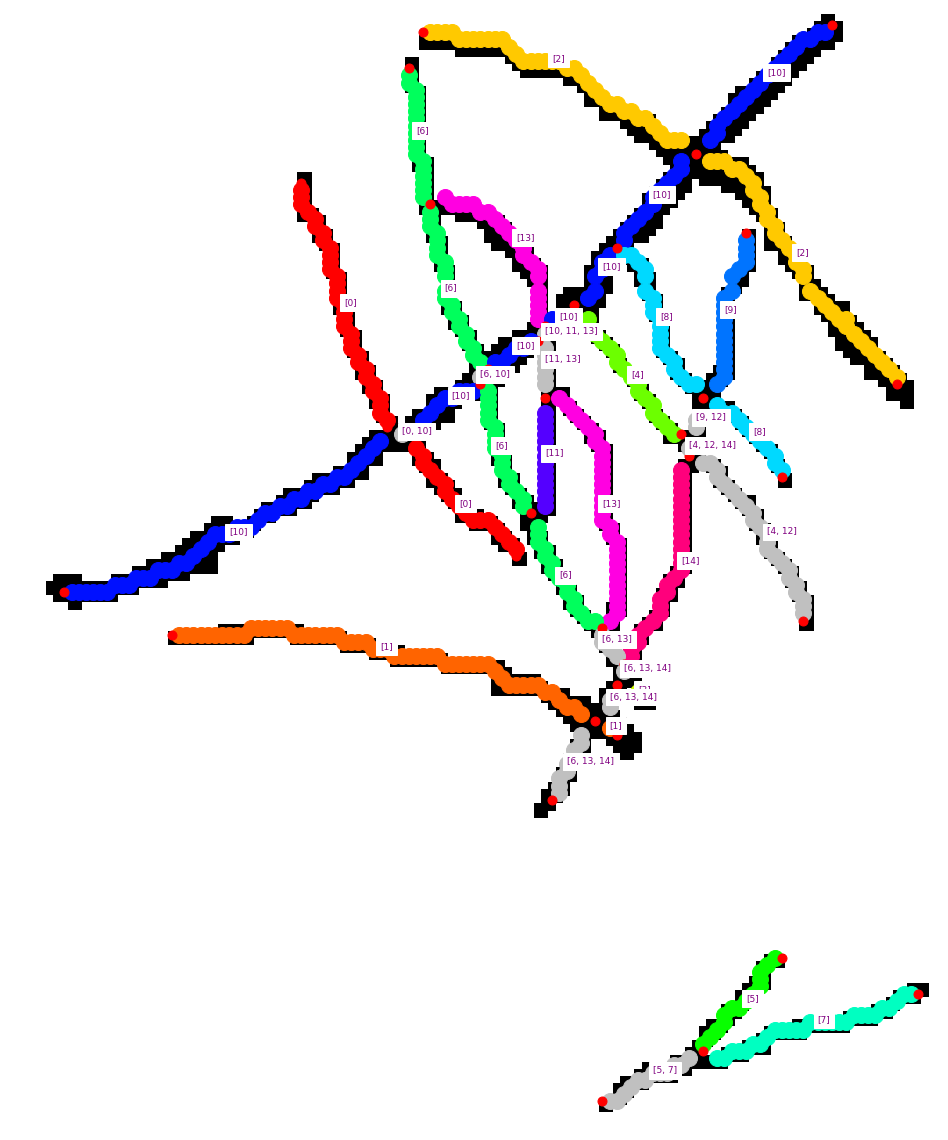
\includegraphics[height=1.5in]{resultImages/field3-t0-2cellBcrop-filtered-phil-s10-v05-antLabeled.png}
        \caption{Peor Resultado de Individualizaci\'on con Phil}
        \label{field3t0filtered1Results-worstPhil}
    \end{subfigure}
    ~ 
    \begin{subfigure}[t]{0.49\textwidth}
        \centering
        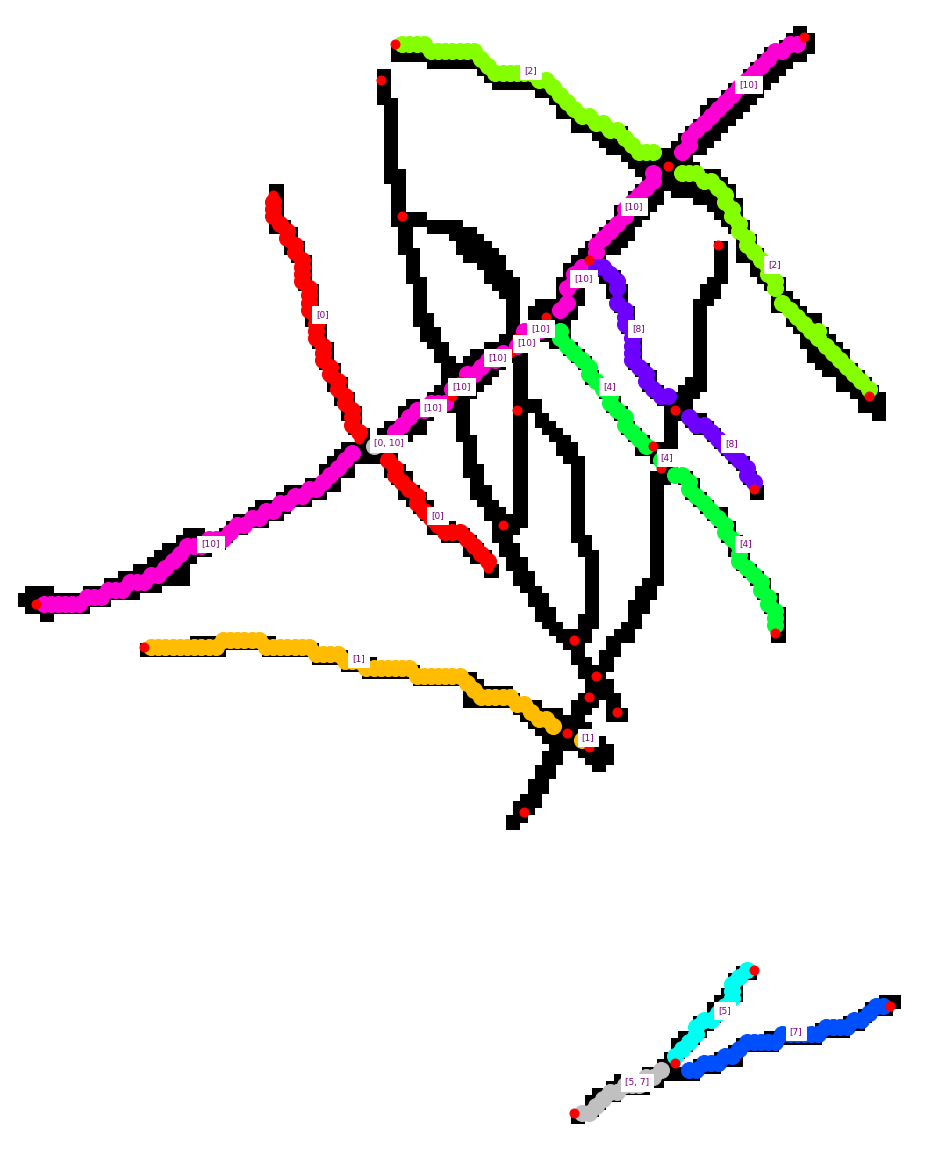
\includegraphics[height=1.5in]{resultImages/field3-t0-2cellBcrop-filtered-phil-s10-v05-exactMatch-antLabeled.png}
        \caption{Filamentos correctamente individualizados en el peor resultado de Phil, identificados con colores}
        \label{field3t0filtered1Results-worstPhilExact}
    \end{subfigure}
    
    \caption{Individualizaci\'on  de filamentos de la figura \ref{fig:field3t0filtered1} correspondiente a la muestra MT-B, realizadas con DeFiNe y Phil. Segmentos marcados en negro representan aristas no asignadas correctamente. f) El mejor resultado con Phil permite encontrar el filamento compuesto por las aristas 8,22,26,27,32,34,36 no encontrado en a) ni en c). }
    \label{fig:field3t0filtered1Results}
\end{figure*}
\clearpage
\newpage

%Valor m\'ax de VI para \ref{tab:field3t0filtered2} es 1.9459.
%N\'umero de filamentos en el {\it Ground Truth} de la figura field3t0 es 5.

La individualizaci\'on de filamentos para la Figura \ref{fig:field3t0filtered2} que representa la muestra MT-C resulta en un empate entre Phil y la configuraci\'on de DeFiNe con 60\textdegree, encontrando 4 de 5 filamentos cada uno, mientras que DeFiNe con 30\textdegree como umbral encuentra s\'olo 3 de 5 filamentos. El filamento faltante en DeFiNe-60\textdegree es el que esta compuesto s\'olo por la arista 4 (Figura \ref{fig:field3t0filtered2Results-d}), mientras que en DeFiNe-30\textdegree se lleva a cabo una asignaci\'on de las aristas 0-3 a un filamento, y de la arista 1 a otro, siendo la combinaci\'on correcta seleccionar la arista 0 por si sola y las aristas 3-1 en conjunto (Figura \ref{fig:field3t0filtered2Results-e}). Similar a lo que realiza Phil, tambi\'en asignado las aristas 3-0 a un filamento, pero a su vez asignando correctamente las aristas 3-1 (Figura \ref{fig:field3t0filtered2Results-f}).  A diferencia de otros resultados, se presenta un solo resultado para Phil ya que las 5 iteraciones arrojan el mismo resultado.


En el caso de Phil, la elecci\'on de las aristas 0-3 para formar un filamento se condice con el comportamiento del algoritmo en buscar caminos/filamentos de mayor longitud que cumplan con el criterio de rectitud. Por otra parte, este caso en un microt\'ubulo puede corresponder a la fusi\'on de 2 microt\'ubulos en uno, denominado {\tt Zippering}, o al nacimiento de un microt\'ubulo a partir de uno existente, llamado {\tt Nucleaci\'on}. Ambas situaciones requieren de informaci\'on adicional para diferenciarlas, como el grosor de los segmentos de filamentos y el \'angulo entre los segmentos de filamentos que se separan del segmento com\'un. La variaci\'on o continuidad del grosor y que el \'angulo mencionado se encuentre en un rango que var\'ia seg\'un el tipo de c\'elula son cr\'iticos para aclarar cual es el caso observado. 

En relaci\'on al an\'alisis de las medidas y las m\'etricas en la tabla \ref{tab:field3t0filtered2}, se mantiene el empate entre DeFiNe-60\textdegree y Phil, con la \'unica diferencia en el tiempo de ejecuci\'on, favorable para Phil. 

\begin{table}[h]
    \centering
    \begin{tabular}{|c|c|c|c|c|c|c|c|c|c|c|}
    \hline
        Algoritmo & VI & TP & FP &TN &FN & Rand	& Jaccard &	Precision &	Recall &	F1 \\ \hline
        Define 30° & 0.5714 & 1 & 1 & 18 & 1 & 0.9047 & 0.3333 & 0.5      & 0.5 & 0.5\\
        Define 60° & 0.4285 & 2 & 1 & 23 & 2 & 0.8928 & 0.4 & 0.6666 & 0.5 & 0.5714\\ 
        Propuesta 0.4285  & 2 & 1 & 23 & 2 & 0.8928 & 0.4 & 0.6666 & 0.5 & 0.5714\\
        \hline
    \end{tabular}
    \caption{Resultados de individualizaci\'on de filamentos para figura \ref{fig:field3t0filtered2}, de la muestra MT-C. El valor m\'aximo de VI en este caso es de 1.9459, ya que el tama\~no del {\it data set} es de 7 aristas. El n\'umero de filamentos en el {\it ground truth} es 5.}
    \label{tab:field3t0filtered2}
\end{table}
\addtocounter{table}{-1}
\begin{table}[h]
    \centering
    \begin{tabular}{|c|c|c|c|c|c|c|}
    \hline
         & \multirow{4}{2cm}{\centering \% Cobertura de Aristas} & \multirow{4}{2cm}{Filamentos Propuestos} & \multirow{4}{2cm}{Filamentos Correctos} & \multirow{4}{2.5cm}{\% Correctos vs Propuestos} & \multirow{4}{2.5cm}{\centering \% Correctos vs {\it Ground Truth}} & \multirow{4}{1.2cm}{\centering Tiempo [seg]} \\
         &  &  &  & & &  \\
        Algoritmo &  &  &  & & &  \\
        &  &  &  & & &  \\ \hline
        Define 30° & 100 & 5 & 3 & 60 & 60 & 2.8262\\
        Define 60° & 100 & 5 & 4 & 80 & 80 & 2.6506\\ 
        Propuesta 100 & 5 & 4 & 80 & 80 & 0.2914\\
        \hline
    \end{tabular}
    \caption{Resultados ({\it Continuaci\'on}) de individualizaci\'on de filamentos para figura \ref{fig:field3t0filtered2}, de la muestra MT-C. El n\'umero de filamentos en el {\it ground truth} es 5.}
\end{table}

\begin{figure*}[h!]
    \centering
    \begin{subfigure}[t]{0.3\textwidth}
        \centering
        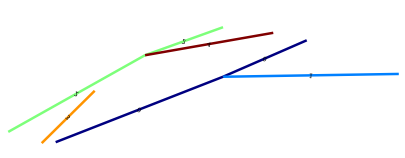
\includegraphics[scale=0.6]{resultImages/field3-t0-2cellBcrop-filtered-2-DeFiNe30.png}
        \caption{Individualizaci\'on mediante DeFiNe con 30\textdegree}
        \label{fig:field3t0filtered2Results-a}
    \end{subfigure}%
    ~ 
    \begin{subfigure}[t]{0.3\textwidth}
        \centering
        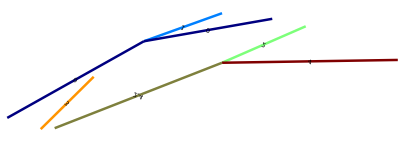
\includegraphics[scale=0.6]{resultImages/field3-t0-2cellBcrop-filtered-2-DeFiNe60.png}
        \caption{Individualizaci\'on mediante DeFiNe con 60\textdegree}
        \label{fig:field3t0filtered2Results-b}
    \end{subfigure}
    ~ 
    \begin{subfigure}[t]{0.3\textwidth}
        \centering
        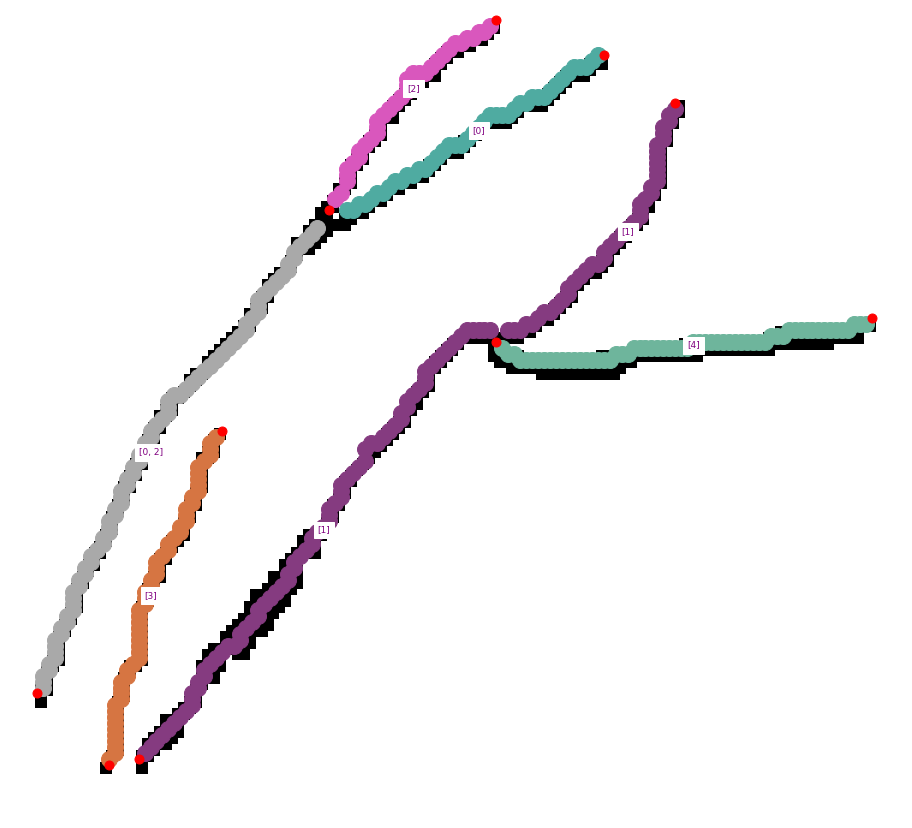
\includegraphics[height=1.5in]{resultImages/field3-t0-2cellBcrop-filtered-2-phil-s1271-v05-antLabeled.png}
        \caption{Individualizaci\'on con Phil}
        \label{fig:field3t0filtered2Results-c}
    \end{subfigure}
    \vskip\baselineskip
    
    \begin{subfigure}[t]{0.3\textwidth}
        \centering
        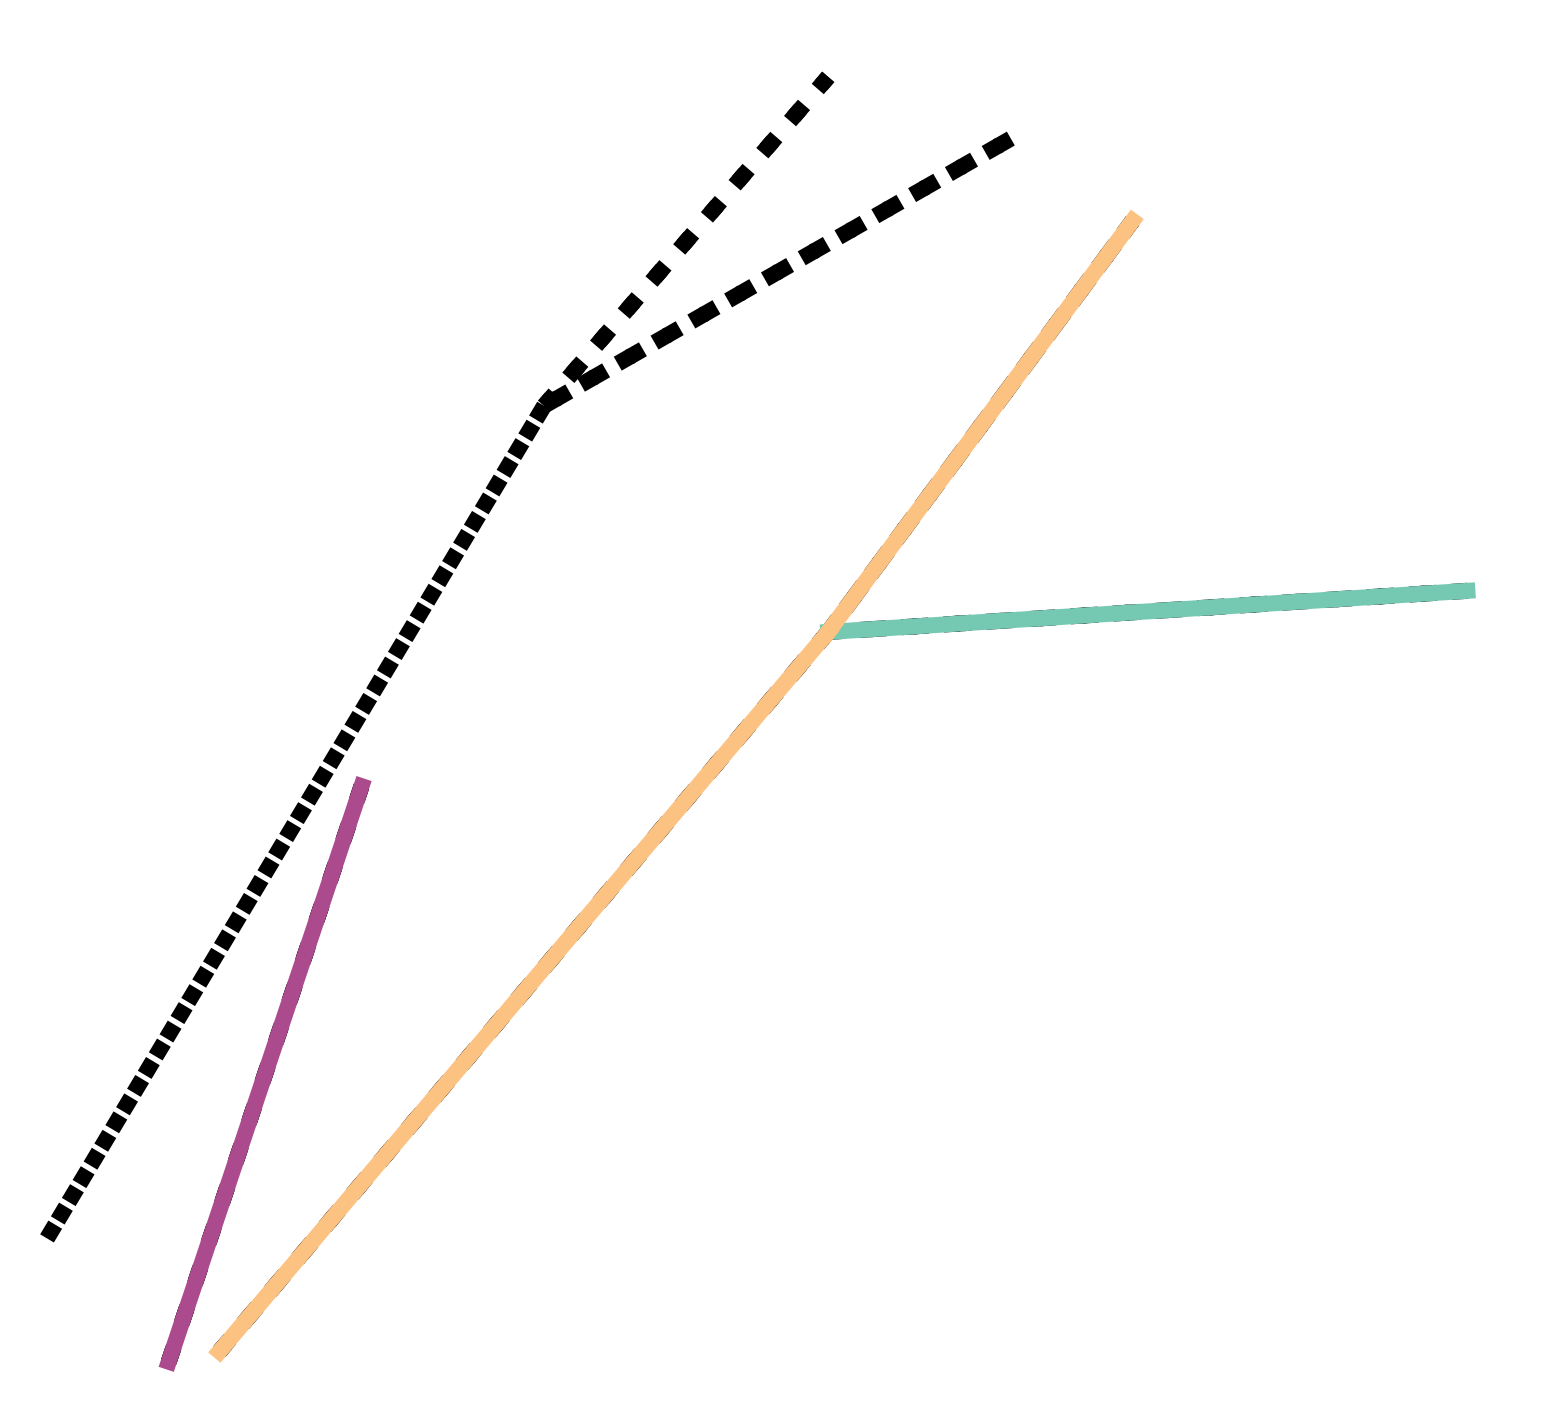
\includegraphics[height=1.5in]{resultImages/field3-t0-2cellBcrop-filtered-2-DeFiNeExactMatch-30.png}
        \caption{Filamentos correctamente individualizados por DeFiNe con 30\textdegree identificados con colores}
        \label{fig:field3t0filtered2Results-d}
    \end{subfigure}%
    ~ 
    \begin{subfigure}[t]{0.3\textwidth}
        \centering
        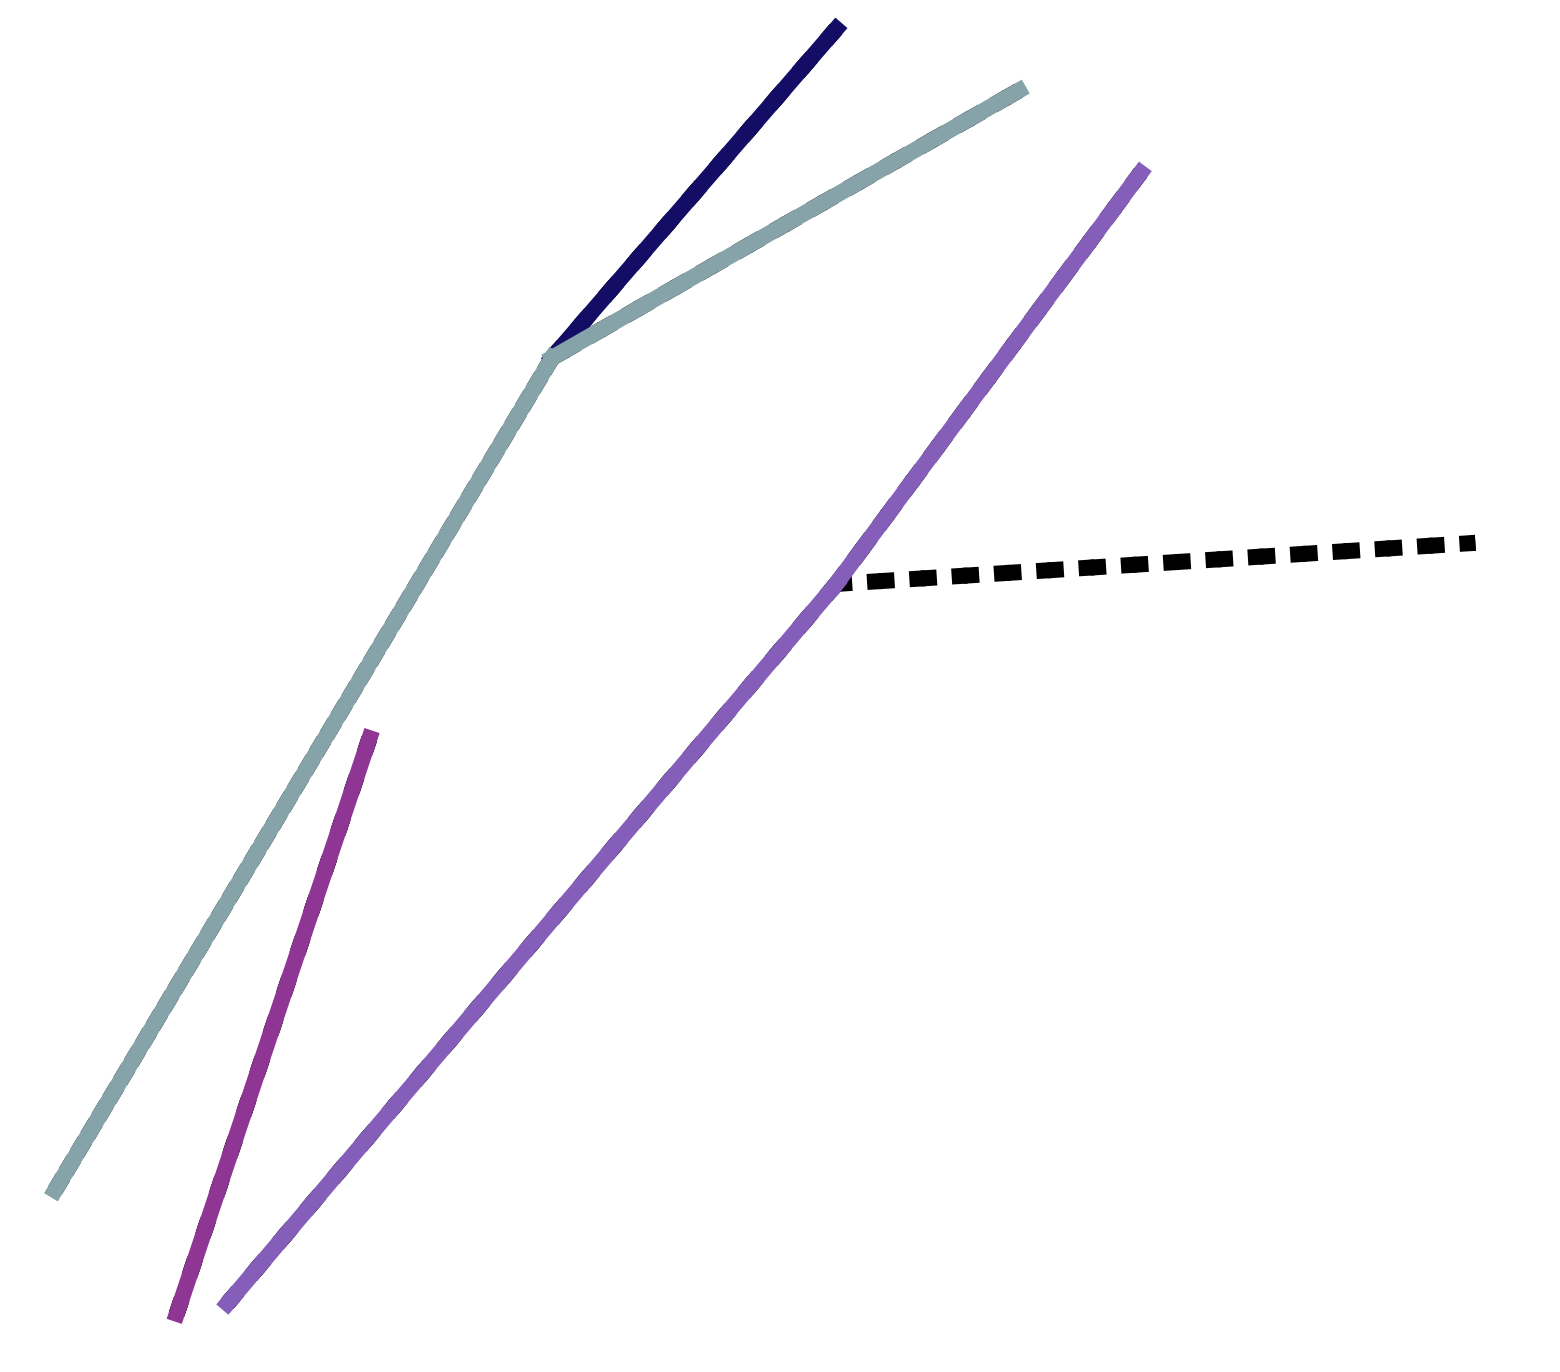
\includegraphics[height=1.5in]{resultImages/field3-t0-2cellBcrop-filtered-2-DeFiNeExactMatch-60.png}
        \caption{Filamentos correctamente individualizados por DeFiNe con 60\textdegree identificados con colores}
        \label{fig:field3t0filtered2Results-e}
    \end{subfigure}
    ~ 
    \begin{subfigure}[t]{0.3\textwidth}
        \centering
        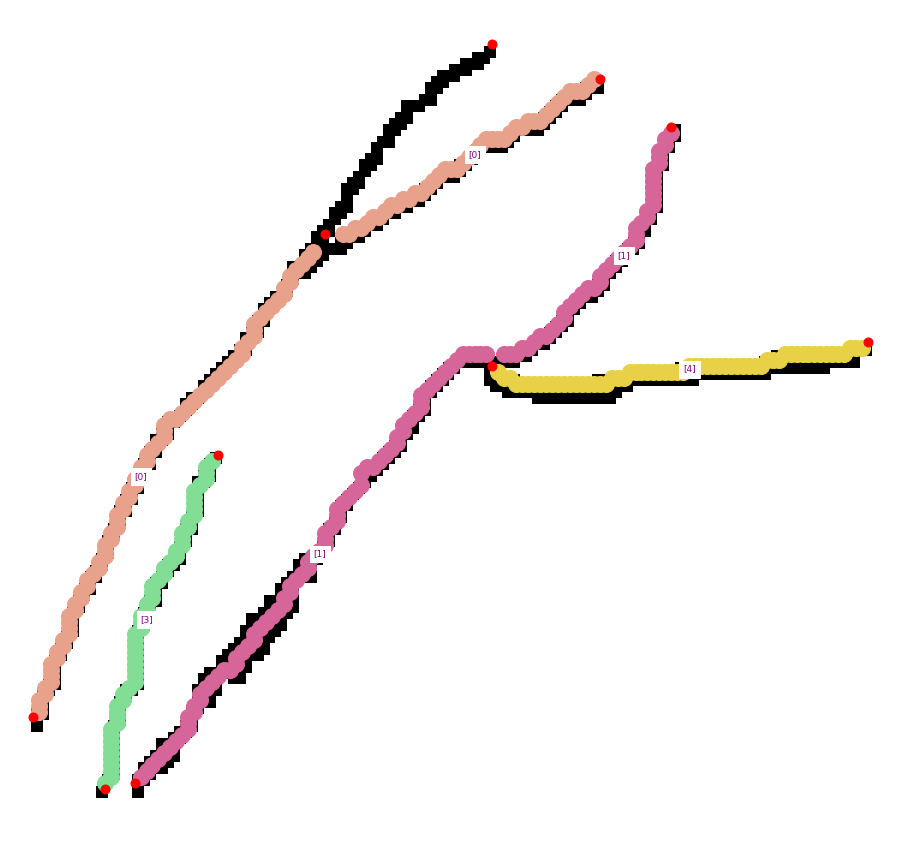
\includegraphics[height=1.5in]{resultImages/field3-t0-2cellBcrop-filtered-2-phil-s1271-v05-exactMatch-antLabeled.png}
        \caption{Filamentos correctamente individualizados por Phil identificados con colores}
        \label{fig:field3t0filtered2Results-f}
    \end{subfigure}
    
    \caption{Individualizaci\'on  de filamentos de la figura \ref{fig:field3t0filtered2} relativa a la muestra MT-C realizadas con DeFiNe y Phil. Segmentos marcados en negro con y sin discontinuidad representan aristas no asignadas correctamente al filamento correspondiente en el {\it ground truth.}.}
    \label{fig:field3t0filtered2Results}
\end{figure*}

\clearpage
\newpage

\subsection{Neuronas}

\section{Resultados Generales}
% t-test para cantidad de filamentos propuestos vs gtruth, y correctos vs gtruth
Para evaluar el desempe\~no general del modelo de optimizaci\'on implementado se calcula la prueba {\it t} de Student o Test-T y la prueba de Kolmog\'orov-Smirnov o prueba K-S sobre los resultados obtenidos por el algoritmo propuesto, DeFiNe, y la individualizaci\'on manual de un experto. En el primer caso se calcula la prueba $t$ de mediciones apareadas independientes, obteni\'endose un {\it p-value} de XXXXX , que al ser mayor que 0.05 no permite rechazar la hip\'otesis nula, por lo que no existe una diferencia estad\'istica significativa entre los resultados del algoritmo propuesto y los de las individualizaciones realizadas por un experto. El resultado de la prueba {\it t} entre el algoritmo propuesto y DeFiNe arroja un resultado similar, con un {\it p-value} de XXXXX, tambi\'en mayor a 0.05, determinando que tampoco existe una diferencia estad\'istica significativa entre los resultados ambos.

%En cuanto a la prueba K-S 

\subsection{Ponderaci\'on de Caracter\'isticas}
\label{subsec:ponderacion}
El modelo de optimizaci\'on desarrollado para la individualizaci\'on de filamentos considera el uso de caracter\'isticas espaciales, topol\'ogicas y geom\'etricas, cuyo uso puede variar dependiendo de la c\'elula representada por el grafo extra\'ido, as\'i como la etapa en el modelo en la cual se aplican. La etapa de construcci\'on de soluciones emplea el \'angulo entre aristas vecinas para definir la posibilidad de elecci\'on que cada hormiga tiene al ir avanzando. En esta etapa tambi\'en se aplica la heur\'istica de asignaci\'on inicial, en la que influye el grado de los nodos para determinar la arista inicial de cada camino. Por su parte, en el m\'etodo de actualizaci\'on de feromonas se usan las caracter\'isticas geom\'etricas como la curvatura del filamento y la diferencia en la magnitud entre segmentos contiguos, agreg\'andose el uso de informaci\'on topol\'ogica obtenida con el algoritmo de centralidad en grafos {\it closeness centrality}, en el caso de las neuronas. En cuanto al m\'etodo de b\'usqueda no local, se utiliza informaci\'on espacial para descartar soluciones que presenten informaci\'on repetida con respecto a otras soluciones.


Dado que las diversas caracter\'isticas utilizadas en el algoritmo propuesto se encuentran en distintos m\'etodos de la metaheur\'istica ACO, no es posible utilizar un \'unico par\'ametro para obtener una ponderaci\'on directa. En cambio, se propone un criterio para su ponderaci\'on basado en otorgar $\frac{1}{3}$ del peso a cada etapa del modelo, distribuyendo aquel valor internamente dependiendo de si la caracter\'istica se utiliza por s\'i sola o en combinaci\'on con otra, as\'i como considerando si el uso es repetitivo durante la ejecuci\'on de la etapa o s\'olo se realiza una vez por etapa. Lo anterior permite establecer la siguiente ponderaci\'on:

\begin{itemize}
    \item Construcci\'on de soluciones: $\frac{100}{n}$\% el grado de los nodos, y el remanente para el \'angulo entre aristas, con $n$ como el n\'umero de aristas.
    \item M\'etodo de b\'usqueda no local: 100\% posici\'on de la arista.
    \item Actualizaci\'on de feromonas: 50\% curvatura, 50\% diferencia de magnitud entre segmentos. En el caso espec\'ifico de las neuronas, corresponde a $33.\overline{3}\%$ curvatura, $33.\overline{3}\%$ diferencia de magnitud entre segmentos y $33.\overline{3}\%$ informaci\'on topol\'ogica de centralidad.
\end{itemize}

Durante la construcci\'on de soluciones, el grado de los nodos s\'olo se utiliza en la heur\'istica de asignaci\'on de la primera arista, por lo que para caminos de una sola arista corresponde a la totalidad de la ponderaci\'on de la etapa. A medida que crece el n\'umero de aristas, su peso va disminuyendo gradualmente al irse traspasando al criterio de \'angulo entre aristas. En cuanto a la diferencia de magnitud entre segmentos, esta se conforma en partes iguales del \'angulo entre segmentos y del uso de la magnitud de los mismos.


En base a los resultados obtenidos mediante la resoluci\'on del modelo de optimizaci\'on es posible observar que la relevancia no se encuentra en encontrar una ponderaci\'on entre propiedades o caracter\'isticas para generar mejores resultados, sino en la incorporaci\'on de m\'as caracter\'isticas que permitan reducir el espacio de b\'usqueda y/o descartar soluciones candidatas que no representen el comportamiento biol\'ogico esperado del filamento en la c\'elula observada.
%La flexibilidad que otorga el modelo 

%30\% \'angulo entre aristas, 3,3\% grado de los nodos, 33,3\% posici\'on, 
%16,6\% curvatura, 8,3\% \'angulo entre segmentos y 8,3\% largo de los segmentos

\section{Discusi\'on}

Observando los resultados obtenidos al individualizar filamentos a partir de im\'agenes sint\'eticas o reales, se tiene que para casos simples existe un comportamiento similar entre el algoritmo propuesto y DeFiNe, con la diferencia de tiempo a favor del algoritmo propuesto. A medida que los casos se complejizan, implicando la existencia de m\'as aristas, el tiempo de resoluci\'on para el algoritmo propuesto se mantiene en rangos de segundos, a diferencia de lo que sucede con DeFiNe. La diferencia entre los tiempos de calculo puede ser atribuida parcialmente a la forma en que se explora el espacio de b\'usqueda, teniendo tambi\'en en cuenta la diferencia entre los lenguajes de programaci\'on utilizados por cada m\'etodo.


El comportamiento del algoritmo propuesto es estable, tendiendo a individualizar los mismos filamentos en cada iteraci\'on, y pudiendo encontrar filamentos que no aparecen en la otra herramienta. Se debe tener en consideraci\'on que este aspecto puede relacionarse con el uso de una ponderaci\'on distinta a la ideal presentada por los autores de DeFiNe, que puede ocasionar la merma en los resultados por aquel m\'etodo.


A su vez, la estabilidad del algoritmo propuesto favorece la experiencia del usuario, ya que evita la sintonizaci\'on de par\'ametros, simplificando el trabajo del experto. Adem\'as, la utilizaci\'on de \'ultiples caracter\'isticas por parte del algoritmo propuesto permite al usuario interactuar con im\'agenes que no sean de buena resoluci\'on.


El uso de curvas de las aristas, en vez de la representaci\'on de estas mediante una l\'inea recta entre 2 nodos no s\'olo aporta m\'as informaci\'on, sino que adem\'as mejora la visualizaci\'on de los resultados. 

